\documentclass[a4paper,11pt]{book}
\usepackage{fullpage}
\usepackage{amsmath}
\usepackage{amssymb}
\usepackage{amstext}
\usepackage{array}
\usepackage{caption}
\usepackage{tikz-qtree,tikz-qtree-compat}
\usepackage{tikz}
\usetikzlibrary{shapes.geometric}
\usetikzlibrary{shapes.multipart}
\usetikzlibrary{shadows}
\usetikzlibrary{positioning}
\usetikzlibrary{trees}
\usetikzlibrary{arrows}

\usepackage{algorithm}
\usepackage{algorithmicx,algpseudocode}

\newlength{\OUmatrixSepWidth}
\newcommand{\OUsetMatrixSepWidth}[1]{%
	\settowidth{\OUmatrixSepWidth}{#1}%
}


\title{Algorithm Design and Analysis (ECS 122A)\\Study Guide}
\author{Davis Computer Science Club\\
	Tutoring Committee
}
\date{Spring Quarter 2015}



\begin{document}

\makeatletter
\begin{titlepage}
	
\noindent \rule{\textwidth}{1pt}

\vspace{1cm}

\noindent {\LARGE \bfseries \@title}

\vspace{1cm}

\noindent \rule{\textwidth}{1pt}

\vspace{1cm}

\noindent	{\Large \@author }

\par\vspace*{\fill}
\begin{flushright}
	Spring Quarter 2015
\end{flushright}
\end{titlepage}

\tableofcontents
\newpage

% 
% ASYMPTOTIC NOTATION
%
\section{Asymptotic Notation}
% Big O
\subsection{O-Notation (Big O)}
\textbf{Notation:} 
$$f(n) \in O(g(n))$$
\textbf{Formal Definition:}\\
For a given function $g(n)$, $O(g(n))$ is the set of functions for which there exists positive constants $c$ and $n_0$ such that $0 \leq f(n) \leq c \cdot g(n)$ for all $n \geq n_0$.
$$
O(g(n)) = \{ f(n) : \exists \text{ } c, n_0 \text{ s.t. } 0 \leq f(n) \leq c \cdot g(n) \text{ } \forall \text{ } n \geq n_0 \}
$$
\textbf{Informal Definition:}\\
The function $g(n)$ is an asymptotic upper bound for the function $f(n)$ if there exists constants $c$ and $n_0$ such that $0 \leq f(n) \leq c \cdot g(n)$ for $n \geq n_0$.\\\\
Another way to perceive Big O notation is that for $f(n) \in O(g(n))$, the function $f$'s asymptotic\footnote{Asymptotic: As given variable approaches infinity.} growth is no faster than that of function $g$'s.\\\\
\textbf{Limit Definition:}
$$ 
\lim\limits_{n \to \infty} \frac{f(n)}{g(n)} < \infty
$$
\newpage
\subsubsection{Example}
\textbf{Prove that asymptotic upper bound of $f(n) = 2n+10$ is $g(n) = n^2$}.
\begin{eqnarray*}
	0 \leq f(n) &\leq& c \cdot g(n) \text{ for } n \geq n_0\\
	0 \leq 2n + 10 &\leq& c \cdot n^2 \text{ for } n \geq n_0
\end{eqnarray*}
Arbitrarily choose $c$ and $n_0$ values. Simplest is to turn one of the variables into the value $1$ and solve. For this example, we will assign the value 1 to $n_0$.
\begin{eqnarray*}
	0 \leq 2n + 10 &\leq& c \cdot n^2 \text{ for } n \geq 1\\
	2(1) + 10 &\leq& c \cdot (1)^2\\
	12 &\leq& c
\end{eqnarray*}
By picking $n_0 = 1$ and $c = 12$, the inequality of $2n+10 \leq 12n^2$ will hold true for all $n \geq 1$. Since there exists a constant $c$ and $n_0$ that fulfill this inequality, we have proven that $f(n) = 2n+10 = O(n^2)$.
\newpage

% Little O
\subsection{o-Notation (Little O)}
\textbf{Notation:}
$$
f(n) \in o(g(n))
$$
\textbf{Formal Definition:}\\
For a given function $g(n)$, $o(g(n))$ is the set  of functions for which every positive constant $c > 0$, there exists a constant $n_0 > 0$ such that $0 \leq f(n) \leq c \cdot g(n)$ for all $n \geq n_0$.
$$
o(g(n)) = \{ f(n) : \exists \text{ } n_0 \text{ s.t. } 0 \leq f(n) \leq c \cdot g(n) \text{ } \forall \text{ } n \geq n_0, c \geq 0 \}
$$
\textbf{Informal Definition:}\\
The function g(n) is an upper bound that is not asymptotically tight. For all positive constant values of $c$, there must exists a constant $n_0$ such that $0 \leq f(n) \leq c \cdot g(n)$ for all $n \geq n_0$. The value of $n_0$ may not depend on n, but may depend on $c$.\\\\
Another way to perceive Little O notation is that for $f(n) \in o(g(n))$, the function $f$'s asymptotic growth is strictly less than that of the function $g$'s. In this sense, Little O can be seen as a ``stronger" bound in comparison to Big O. By proving that a function is an element of Little O, it also proves that the function is an element of Big O.\\\\
\textbf{Limit Definition:}
$$
\lim\limits_{n\to\infty} \frac{f(n)}{g(n)} = 0
$$
\newpage
\subsubsection{Example}
\textbf{Prove that $f(n) = 2n$ has an upper bound $o(n^2)$.}
\begin{eqnarray*}
	0 \leq c \cdot g(n) &\leq& f(n) \text{ for } n \geq n_0\\
	0 \leq c \cdot 2n &\leq& n^2 \text{ for } n \geq n_0\\
	2c &\leq& n \text{ for } n \geq n_0\\
	2c &\leq& n_0
\end{eqnarray*}
For Little O to hold true, the inequality needs to hold true for all $c > 0$ and for all $n > n_0$. From simplifying the inequality, we assert that the inequality will hold true as long as the value of $n_0$ is twice the value of $c$. Given that they are both constants, then there exists a constant value of $n_0$ for all positive constant $c$ that fulfill this inequality.\\\\
Another method to solve this problem is to use the limit definition.
\begin{eqnarray*}
	&\lim\limits_{n\to\infty}& \frac{2n}{n^2}\\
	&\lim\limits_{n\to\infty}& \frac{2}{n} = 0	
\end{eqnarray*}

\subsubsection{Example}
\textbf{Prove that $f(n) = 2n^2$ does not have the upper bound $o(n^2)$.}
\begin{eqnarray*}
	0 \leq c \cdot g(n) &\leq& f(n) \text{ for } n \geq n_0\\
	0 \leq c \cdot 2n^2 &\leq& n^2 \text{ for } n \geq n_0\\
	2c &\leq& 1\text{ for } n \geq n_0
\end{eqnarray*}
For a function to have the Little O bound, the inequality must hold true for all positive $c$. However, simplification of the inequality asserts that the inequality will only hold true for all $c < \frac{1}{2}$. Therefore, $f(n) = 2n^2$ does not have the upper bound $o(n^2)$.
\newpage

% Big Omega
\subsection{$\Omega$-Notation (Big Omega)}
\textbf{Notation:}
$$
f(n) \in \Omega(g(n))
$$
\textbf{Formal Definition:}\\
For a given function $g(n)$, $\Omega(g(n))$ is the set of functions for which there exists positive constants $c$ and $n_0$ such that $0 \leq c \cdot g(n) \leq f(n)$ for all $n \geq n_0$.
$$
\Omega(g(n)) = \{ f(n) : \exists \text{ } c, n_0 \text{ s.t. } 0 \leq c \cdot g(n) \leq f(n) \text{ } \forall \text{ } n \geq n_0 \}
$$
\textbf{Informal Definition:}\\
The function $g(n)$ is an asymptotic lower bound for the function $f(n)$ if there exists constants $c$ and $n_0$ such that $0 \leq c \cdot g(n) \leq f(n)$ for $n \geq n_0$.\\\\
\textbf{Limit Definition:}
$$
\lim\limits_{n \to \infty} \frac{f(n)}{g(n)} > 0
$$
\newpage
\subsubsection{Example}
\textbf{Prove that the asymptotic lower bound of $f(n) = 8n^2$ is $g(n) = n$.}
\begin{eqnarray*}
	0 \leq c \cdot g(n) &\leq& f(n) \text{ for } n \geq n_0\\
	0 \leq c \cdot n &\leq& 8n^2 \text{ for } n \geq n_0
\end{eqnarray*}
Arbitrarily choose $c$ and $n_0$ values. Simplest is to turn one of the variables into the value $1$ and solve. For this example, we will assign the value 1 to $c$.
\begin{eqnarray*}
	0 \leq n &\leq& 8n^2 \text{ for } n \geq n_0\\
		   (n_0) &\leq& 8(n_0)^2\\
		   1 &\leq& 8n_0\\
		   \frac{1}{8} &\leq& n_0
\end{eqnarray*}
By picking $n_0 = 1$ and $c = 1$, the inequality of $n \leq 8n^2$ will hold true for all $n \geq 1$. Since there exists a constant $c$ and $n_0$ that fulfill this inequality, we have proven that $f(n) = n^2 = \Omega(n)$.
\newpage

% Little Omega
\subsection{$\omega$-Notation (Little Omega)}
\textbf{Notation:}
$$
f(n) \in \omega(g(n))
$$
\textbf{Formal Definition:}\\
For a given function $g(n)$, $\omega(g(n))$ is the set  of functions for which every positive constant $c > 0$, there exists a constant $n_0 > 0$ such that $0 \leq c \cdot g(n) \leq f(n)$ for all $n \geq n_0$.
$$
\omega(g(n)) = \{ f(n) : \exists \text{ } n_0 \text{ s.t. } 0 \leq c \cdot g(n) \leq f(n) \text{ } \forall \text{ } n \geq n_0, c \geq 0 \}
$$
\textbf{Informal Definition:}\\
The function g(n) is a lower bound that is not asymptotically tight. For all positive constant values of $c$, there must exists a constant $n_0$ such that $0 \leq c \cdot g(n) \leq f(n)$ for all $n \geq n_0$. The value of $n_0$ may not depend on n, but may depend on $c$.\\\\
Another way to perceive Little $\omega$ notation is that for $f(n) \in \omega(g(n))$, the function $f$'s asymptotic growth is strictly greater than that of the function $g$'s. In this sense, Little $\omega$ can be seen as a ``stronger" bound in comparison to Big $\Omega$. By proving that a function is an element of Little $\omega$, it also proves that the function is an element of Big $\Omega$.\\\\
\textbf{Limit Definition:}
$$
\lim\limits_{n\to\infty} \frac{f(n)}{g(n)} = \infty
$$
\newpage

% Theta
\subsection{$\Theta$-notation}
\textbf{Notation:}\\
$$
f(n) \in \Theta(g(n))
$$
\textbf{Formal Definition:}\\
For a given function $g(n)$, $\Theta(g(n))$ is the set of functions for which there exists positive constants $c_1$, $c_2$, and $n_0$ such that $0 \leq c_1 \cdot g(n) \leq f(n) \leq c_2 \cdot g(n)$ for all $n \geq n_0$.
$$
\Theta(g(n)) = \{ f(n) : \exists \text{ } c_1, c_2, n_0 \text{ s.t. } 0 \leq c_1 \cdot g(n) \leq f(n) \leq c_2 \cdot g(n) \text{ } \forall \text{ } n \geq n_0 \}
$$
\textbf{Informal Definition:}\\
The function g(n) is an asymptotic tight bound for the function f(n) if there exists constants $c_1$, $c_2$, and $n_0$ such that $0 \leq c_1 \cdot g(n) \leq f(n) \leq c_2 \cdot g(n)$ for $n \geq n_0$.\\\\
\textbf{Limit Definition:}\\
$$
\lim\limits_{n\to\infty} \frac{f(n)}{g(n)} \in \mathbb{R}_{>0}
$$
\newpage

%
% RECURRENCE RELATIONS
%
\chapter{Recurrence Relations}

\section{Recurrence Relations}
A recurrence relation is an equation that recursively defines a sequence of values. After the initial terms are given, each subsequent term is defined as a function of the previous terms.

\subsection{Fibonacci}
Fibonacci is an example of a recurrence relation.
$$
F_n = \begin{cases}
	F_{n-1} + F_{n-2}, &  n \geq 2\\
	1, & n = 1\\
	0, & n = 0
\end{cases}
$$
The first two terms are defined while the subsequent terms are a function of the two previous.

\subsection{Solving Recurrence Relations}
\begin{itemize}
	\item Substitution Method
	\item Recursion-Tree Method
	\item Master Method
\end{itemize}

\subsection{Substitution Method}
\begin{enumerate}
	\item Guess the bounds.
	\item Apply mathematical induction to prove the bounds. 
\end{enumerate}

\subsubsection{Example}
\textbf{Find the asymptotic upper bound for the following function:}
$$
T(n) \begin{cases}
	2T(n-1) + 1, & n \geq 1\\
	1, & n = 0
	\end{cases}
$$
\textbf{Guess}
$$T(n) \in O(2^n)$$
\textbf{Inductive Basis}
\begin{eqnarray*}
	T(0) &=& 2^0\\
	&=& 1
\end{eqnarray*}
\textbf{Inductive Hypothesis}\\
Assume that $T(n) = 2^n$ holds true for all $n = k$.\\\\
\textbf{Inductive Step}
\begin{align*}
T(n)	&=	2T(n-1) + 1						&& \text{Base equation}\\
		&= 	2T((k+1) - 1) + 1				&& \text{Substitute n with } k+1\\
		&=	2T(k) + 1						&& \text{Simplify parameters to T(n)}\\
		&=  2(2^k) + 1						&& \text{Substitute T(n) with inductive hypothesis}\\
		&=  2^{k+1} + 1						&& \text{Property of exponents}\\
&											&& \text{Q.E.D}
\end{align*}

%
% DIVIDE AND CONQUER
%
\chapter{Divide and Conquer Paradigm}
\newpage

\section{Steps}

\begin{enumerate}
	\item \textbf{Divide} the problem into a number of independent subproblems.
	\item \textbf{Conquer} the subproblems by solving them recursively. 
	\item \textbf{Combine} the solutions of the subproblems into the solution of the original problem. 
\end{enumerate}
\newpage


\section{Case Study: Fibonacci Sequence}

\subsection*{Theorem}

\subsubsection*{Fibonacci Sequence Starting with 0}
Sequence: 0, 1, 1, 2, 3, 5, 8, 13, 21, 34, ...
\[
\begin{bmatrix}
F_{n}\\
F_{n-1}
\end{bmatrix}
=
\begin{bmatrix}
1 & 1\\
1 & 0
\end{bmatrix}^{n-1}
\begin{bmatrix}
F_{0}\\
F_{1}
\end{bmatrix}
\]

\subsubsection*{Fibonacci Sequence Starting with 1}
Sequence: 1, 1, 2, 3, 5, 8, 13, 21, 34, ...
\[
\begin{bmatrix}
F_{n}\\
F_{n-1}
\end{bmatrix}
=
\begin{bmatrix}
1 & 1\\
1 & 0
\end{bmatrix}^{n-1}
\begin{bmatrix}
F_{1}\\
F_{2}
\end{bmatrix}
\]

\subsection*{Derivation}
\begin{eqnarray*}
\begin{bmatrix}
	F_n\\
	F_{n-1}
\end{bmatrix}	
&=&
\begin{bmatrix}
	1 & 1\\
	1 & 0
\end{bmatrix}
\begin{bmatrix}
	F_{n-1}\\
	F_{n-2}
\end{bmatrix}\\
&=&
\begin{bmatrix}
	1 & 1\\
	1 & 0
\end{bmatrix}
\begin{bmatrix}
	1 & 1\\
	1 & 0
\end{bmatrix}
\begin{bmatrix}
	F_{n-2}\\
	F_{n-3}
\end{bmatrix}\\
&=&
\begin{bmatrix}
	1 & 1\\
	1 & 0
\end{bmatrix}
\begin{bmatrix}
	1 & 1\\
	1 & 0
\end{bmatrix}
\begin{bmatrix}
	1 & 1\\
	1 & 0
\end{bmatrix}
\begin{bmatrix}
	F_{n-3}\\
	F_{n-4}
\end{bmatrix}\\
&=&
\begin{bmatrix}
	1 & 1\\
	1 & 0
\end{bmatrix}^4
\begin{bmatrix}
	F_{n-4}\\
	F_{n-5}
\end{bmatrix}\\
&=&
\begin{bmatrix}
	1 & 1\\
	1 & 0
\end{bmatrix}^{n-1}
\begin{bmatrix}
	F_{0}\\
	F_{1}
\end{bmatrix}\\
\end{eqnarray*}
$$\text{To verify, let's choose } n = 5$$
\begin{eqnarray*}
	\begin{bmatrix}
		F_{5}\\
		F_{4}
	\end{bmatrix}
	&=&
	\begin{bmatrix}
		1 & 1\\
		1 & 0
	\end{bmatrix}^4
	\begin{bmatrix}
		F_{0}\\
		F_{1}
	\end{bmatrix}\\
		&=&
		\begin{bmatrix}
			5 & 3\\
			3 & 2
		\end{bmatrix}
		\begin{bmatrix}
			0\\
			1
		\end{bmatrix}\\
	&=&
	\begin{bmatrix}
		3\\
		2
	\end{bmatrix}
\end{eqnarray*}
$$
\text{The fifth Fibonacci number (assuming that the sequence starts at 0) is 3.}
$$

\subsection*{Recurrence Relation}
$$T(n) = T(\frac{n}{2}) + O(1)$$

\subsection*{Complexity}
$$T(N) \in \Theta(lg(n))$$
\newpage

\section{Case Study: Merge Sort}

\subsection*{Steps}

\begin{enumerate}
	\item \textbf{Divide} the list of n elements into two sublists with $\frac{n}{2}$ elements each.
	\item \textbf{Conquer} the sublists by sorting the two sublists recursively using merge sort. When the sublists are of size 1, it becomes sorted.
	\item \textbf{Combine} the elements of the two sublists by mering them in a sorted sequence.
\end{enumerate}

\subsection*{Recurrence Relation}
$$
T(n) = \begin{cases}
2T\left(\frac{n}{2}\right) + cn, & n \geq 2\\
c, & n = 1
\end{cases}
$$

\subsection*{Complexity}
$$
T(n) = \Theta(n \cdot lg(n))
$$

%\subsection{Example}
%\textbf{Show the steps of sorting the following list using merge sort: $\{ 13, 82, 72, 100, 25, 48, 71, 14 \}$}
\newpage

\section{Case Study: Maximum Subarray}

\subsection*{Steps}

\begin{enumerate}
	\item Divide the array in half into two subarrays (left subarray and right subarray).
	\item Recursively repeat this process until each subarray consists of only one element. At this point, the maximum sum of each subarray is the single element.
	\item Calculate the maximum sum for the cross section.
	\begin{enumerate}
		\item Start from the mid-point of the subarray.
		\item Sum up all numbers from the mid-point to the first element. Whenever the sum exceeds its previous value, that value becomes the left sum.
		\item Sum up all numbers from the mid-point+1 to the last element. Whenever the sum exceeds its previous value, that values becomes the right sum.
		\item The summation of the left sum and the right sum becomes the maximum sum for the cross section. Note: If all the elements in the subarrays are negative, then the left and right sum will return 0 by default.
	\end{enumerate}
	\item Compare the maximum sum from the left array, right array, and cross section. The largest of the three get returned.
\end{enumerate}

\subsection*{Recurrence Relation}
$$
T(n) = 2T(\frac{n}{2}) + \Theta(n)
$$

\subsection*{Complexity}
$$
T(n) \in \Theta(n \cdot lg(n))
$$

\newpage

\subsection{Example}
\textbf{Find the maximum subarray of the following array: $\{-2, 1, -3, 4, -1, 2, 1, -5, 4 \} $ }

\subsubsection*{Divide}
\begin{figure}[h]
	\centering
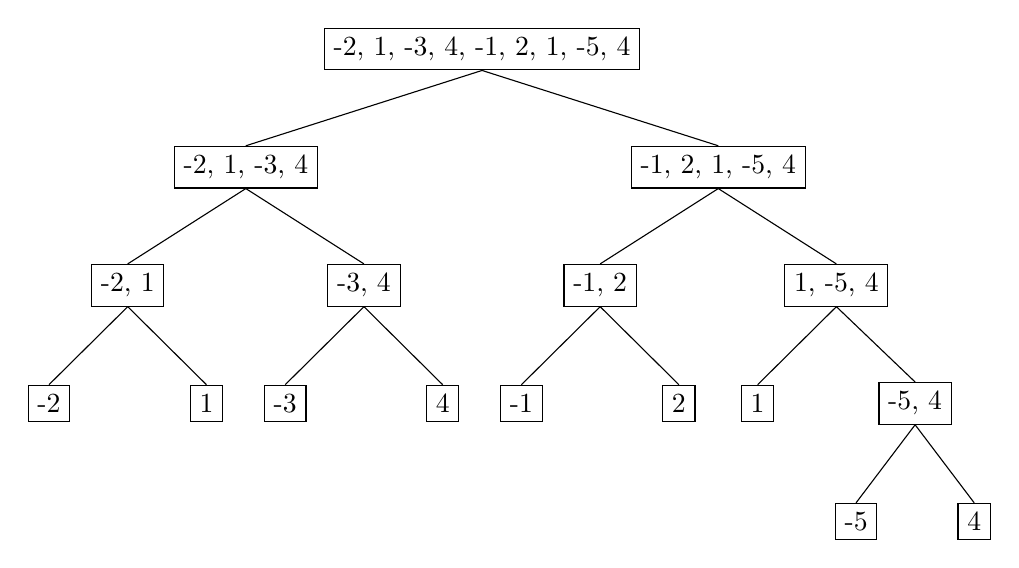
\begin{tikzpicture}[level/.style={sibling distance=60mm/#1}]
	\node [rectangle,draw] {-2, 1, -3, 4, -1, 2, 1, -5, 4}
		child {
			node [rectangle,draw] (a) {-2, 1, -3, 4}
				child {
					node [rectangle,draw] {-2, 1}
						child {
							node [rectangle, draw] {-2}
						}
						child {
							node [rectangle, draw] {1}
						}
				}
				child {
					node [rectangle,draw]{-3, 4}
					child {
						node [rectangle, draw] {-3}
					}
					child {
						node [rectangle, draw] {4}
					}
				}
		}
		child {
			node [rectangle,draw] (b) {-1, 2, 1, -5, 4}
				child {
					node [rectangle,draw]  {-1, 2}
						child {
							node [rectangle, draw] {-1}
						}
						child {
							node [rectangle, draw] {2}
						}
				}
				child {
					node [rectangle,draw]  {1, -5, 4}
						child {
							node [rectangle, draw]  {1}
						}
						child {
							node [rectangle, draw] {-5, 4}
								child {
									node [rectangle, draw] {-5}
								}
								child {
									node [rectangle, draw] {4}
								}
						}
				}
		};
\end{tikzpicture}
\end{figure}

\subsubsection*{Combine}
\begin{table}[h]
	\centering
	\begin{tabular}{| >{$}c<{$} | >{$}c<{$} |  >{$}c<{$} | >{$}c<{$} | >{$}c<{$} | >{$}c<{$} | >{$}c<{$} |}
		\hline
		\text{Depth}
			&	\text{Left Subarray}
			&	\text{Right Subarray}	
			&	\text{Max(Left)}	
			&	\text{Max(Right)}	
			&	\text{Max(Cross)}
			&	\text{Return}\\
		\hline
		4		
			&	\{ -5 \}	
			&	\{ 4 \}
			& 	-5
			&	4
			&	4
			&	4\\
		\hline
		3
			&	\{ -2 \}
			&	\{ 1 \}
			&	-2
			&	1
			&	1
			&	1\\
		\hline
			&	\{ -3 \}
			&	\{ 4 \}
			&	-3
			&	4
			&	4
			&	4\\
		\hline
			&	\{ -1 \}
			&	\{ 2 \}
			&	-1
			&	2
			&	2
			&	2\\
		\hline
			&	\{ 1 \}
			&	\{ -5, 4 \}
			& 	1
			&	4
			&	4
			&	4\\
		\hline
		2
			&	\{ -2, 1\}
			&	\{ -3, 4\}
			&	1
			&	4
			&	1
			&	4\\
		\hline
			&	\{ -1, 2 \}
			&	\{ 1, -5, 4 \}
			&	2
			&	4
			&	3
			&	4\\
		\hline
		1
			&	\{ -2, 1, -3, 4 \}
			&	\{ -1, 2, 1, -5, 4 \}
			&	4
			&	4
			&	6
			&	6\\
		\hline
	\end{tabular}
\end{table}
$$
\text{The maximum sum is 6 from indices 3 to 6.}
$$

\subsubsection*{Visualization of Finding the Max of Cross Section}
Taking depth = 1 with left subarray = $\{ -2, 1, -3, 4 \}$ and right subarray = $\{ -1, 2, 1, -5, 4 \}$.

\begin{minipage}[t]{0.5\linewidth}
	$$
	\text{Cross Section Left Sum}
	$$
	$$
	\{ -2, 1, -3, 4, \underbrace{-1}_{\text{Mid}}, 2, 1, -5, 4 \}
	$$
	$$
	\{ -2, 1, -3, 4, \underbrace{-1}_{\text{-1}}, 2, 1, -5, 4 \}
	$$
	$$
	\{ -2, 1, -3, \underbrace{4, -1}_{\text{3}}, 2, 1, -5, 4 \}
	$$
	$$
	\{ -2, 1, \underbrace{-3, 4, -1}_{\text{0}}, 2, 1, -5, 4 \}
	$$
	$$
	\{ -2, \underbrace{1, -3, 4, -1}_{\text{1}}, 2, 1, -5, 4 \}
	$$
	$$
	\{ \underbrace{-2, 1, -3, 4, -1}_{\text{-1}}, 2, 1, -5, 4 \}
	$$
	$$\text{Max Left Sum} = 3$$
\end{minipage}
\begin{minipage}[t]{0.5\linewidth}
	$$
		\text{Cross Section Right Sum}
	$$
	$$
	\{ -2, 1, -3, 4, -1, \underbrace{2}_{\text{Mid + 1}}, 1, -5, 5 \}
	$$
	$$
	\{ -2, 1, -3, 4, -1, \underbrace{2}_{\text{2}}, 1, -5, 5 \}
	$$
	$$
	\{ -2, 1, -3, 4, -1, \underbrace{2, 1}_{\text{3}}, -5, 5 \}
	$$
	$$
	\{ -2, 1, -3, 4, -1, \underbrace{2, 1, -5}_{\text{-2}}, 4 \}
	$$
	$$
	\{ -2, 1, -3, 4, -1, \underbrace{2, 1, -5, 4}_{\text{2}} \}
	$$
	$$
	\text{Max Right Sum} = 3
	$$
\end{minipage}




%
% GREEDY ALGORITHM
%
\chapter{Greedy Algorithm}
\newpage

\section{Properties}

\subsection*{Greedy Choice}
A globally optimal solution can be arrived at by making a locally optimal (greedy) choice.

\subsection*{Optimal Substructure Property}
An optimal solution to the problem contains within it optimal solution to the subproblems.

\newpage


\section{Case Study: Activity-Selection}
\newpage

\section{Case Study: Huffman Coding}

\subsection{Formal Problem Statement}
Let A be defined as the set of alphabets. ( $A = \{ a_0, a_1, a_2, ..., a_n \}$ )\\
Let W be defined as the set of weights for which $w_i = \text{Weight}(a_i)$.  ($W = \{ w_0, w_1, w_2, ..., w_n \}$)
Let C be defined as the set of (binary) codewords for which $c_i = \text{CodeWord}(a_i)$.\\\\
Assume there exists $n$ alphabets, each with a weight $w_i$. Find and define the codewords $c_i$ for each respective alphabet $a_i$ such that $\sum\limits_{i=0}^{n} w_i \cdot length(c_i)$ is the smallest possible.

\subsection{Informal Problem Statement}
Given a set of symbols and their weights (probabilities), find a prefix-free binary code with minimum expected codeword length.

\subsection{Greedy Choice}
Choose the two alphabets with the lowest weight. 

\subsection{Steps}
\begin{enumerate}
	\item Pick two letters $x$ and $y$ from the alphabet A with the lowest frequencies or weight $w_i$.
	\item Create a subtree with $x$ and $y$ as leaves. We will define the root as $z$.
	\item The frequency or weight of node $z$ will be define as $w_z = w_x + w_y$.
	\item Remove $x$ and $y$ from alphabet.\\
		$ A^\prime = A - \{ x, y \}$
	\item Insert $z$ into the alphabet.\\
		$ A^\prime = A + \{ z \} $
	\item Repeat this process until the set of alphabets $A$ consists of only one alphabet.
\end{enumerate}

\newpage

\subsection{Example}
\textbf{Let $A = \{ a, b, c, d, e \}$ and $W = \{ 30, 16, 6, 15, 35 \}$. Find their corresponding Huffman codes.}

\subsubsection*{Merge $c$ and $d$}
\begin{minipage}{0.35\linewidth}
	\flushleft
	\begin{tabular}{| c | c |}
		\hline
		Alphabet	&	Weight\\
		\hline
		e			&	35\\
		\hline
		a			&	30\\
		\hline
		b			&	16\\
		\hline
		d			&	15\\
		\hline
		c			&	6\\
		\hline
	\end{tabular}
\end{minipage}
\qquad
\begin{minipage}{0.65\linewidth}
	\centering
	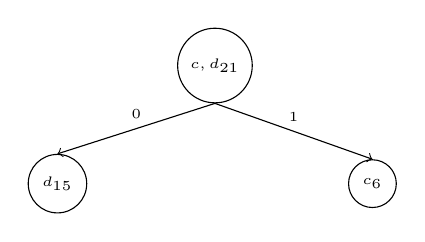
\begin{tikzpicture}[level/.style={sibling distance=40mm/#1}]
	\node [circle,draw] {\tiny$c,d_{21}$}
	child {
		node [circle,draw] {\tiny$d_{15}$}
		edge from parent [->] node [above] {\tiny 0}
	}
	child {
		node [circle,draw] {\tiny$c_6 $}
		edge from parent [->] node [above] {\tiny 1}
	};
	\end{tikzpicture}
\end{minipage}


\subsubsection*{Merge $c,d$ and $b$}
	\begin{minipage}{0.35\linewidth}
		\flushleft
		\begin{tabular}{| c | c |}
			\hline
			Alphabet	&	Weight\\
			\hline
			e			&	35\\
			\hline
			a			&	30\\
			\hline
			c,d			&	21\\
			\hline
			b			&	16\\
			\hline
		\end{tabular}
	\end{minipage}
	\qquad
\begin{minipage}{0.65\linewidth}
	\centering
	\begin{tikzpicture}[level/.style={sibling distance=60mm/#1}]
	\node [circle,draw] {\tiny$b,c,d_{37}$}
	child {
		node [circle,draw] {\tiny$c,d_{21}$}
		child {
			node [circle,draw] {\tiny$d_{15}$}
			edge from parent [->] node [above] {\tiny 0}
		}
		child {
			node [circle, draw] {\tiny$c_{6}$}
			edge from parent [->] node [above] {\tiny 1}
		}
		edge from parent [->] node [above] {\tiny 0}
	}
	child {
		node [circle,draw] {\tiny$b_{16} $}
		edge from parent [->] node [above] {\tiny 1}
	};
	\end{tikzpicture}
\end{minipage}

\subsubsection*{Merge $e$ and $a$}
\begin{minipage}{0.35\linewidth}
\flushleft
	\begin{tabular}{| c | c |}
		\hline
		Alphabet	&	Weight\\
		\hline
		b,c,d			&	37\\
		\hline
		e			&	35\\
		\hline
		a			&	30\\
		\hline
	\end{tabular}
\end{minipage}
\qquad
\begin{minipage}{0.30\linewidth}
	\centering
	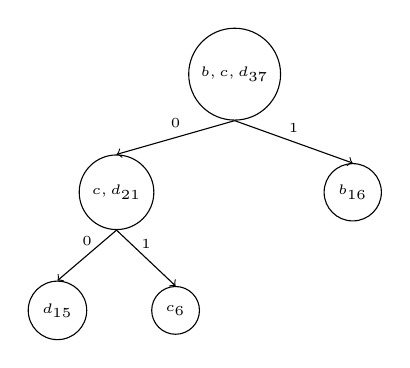
\begin{tikzpicture}[level/.style={sibling distance=30mm/#1}]
	\node [circle,draw] {\tiny$b,c,d_{37}$}
	child {
		node [circle,draw] {\tiny$c,d_{21}$}
		child {
			node [circle,draw] {\tiny$d_{15}$}
			edge from parent [->] node [above] {\tiny 0}
		}
		child {
			node [circle, draw] {\tiny$c_{6}$}
			edge from parent [->] node [above] {\tiny 1}
		}
		edge from parent [->] node [above] {\tiny 0}
	}
	child {
		node [circle,draw] {\tiny$b_{16} $}
		edge from parent [->] node [above] {\tiny 1}
	};
	\end{tikzpicture}
\end{minipage}
\begin{minipage}{0.30\linewidth}
	\centering
	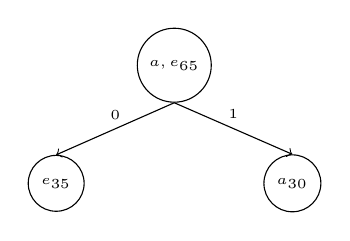
\begin{tikzpicture}[level/.style={sibling distance=30mm/#1}]
	\node [circle,draw] {\tiny$a,e_{65}$}
	child {
		node [circle,draw] {\tiny$e_{35}$}
		edge from parent [->] node [above] {\tiny 0}
	}
	child {
		node [circle,draw] {\tiny$a_{30} $}
		edge from parent [->] node [above] {\tiny 1}
	};
	\end{tikzpicture}
\end{minipage}


\subsubsection*{Merge $a,b,c,d$ and $e$}
\begin{minipage}{0.35\linewidth}
	\flushleft
	\begin{tabular}{| c | c |}
		\hline
		Alphabet	&	Weight\\
		\hline
		a,e			&	65\\
		\hline
		b,c,d		&	37\\
		\hline
	\end{tabular}
\end{minipage}
\qquad
\begin{minipage}{0.65\linewidth}
\centering
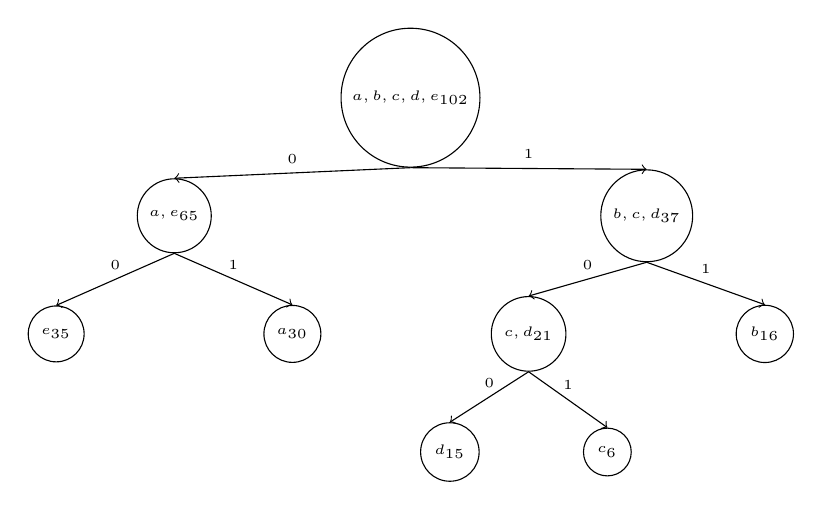
\begin{tikzpicture}[level/.style={sibling distance=60mm/#1}]
	\node [circle,draw] {\tiny$a,b,c,d,e_{102}$}
	child {
		node [circle,draw] {\tiny$a,e_{65}$}
		child {
			node [circle,draw] {\tiny$e_{35}$}
			edge from parent [->] node [above] {\tiny 0}
		}
		child {
			node [circle, draw] {\tiny$a_{30}$}
			edge from parent [->] node [above] {\tiny 1}
		}
		edge from parent [->] node [above] {\tiny 0}
	}
	child {
		node [circle,draw] {\tiny$b,c,d_{37} $}
		child {
			node [circle,draw] {\tiny $c,d_{21}$ }
			child {
				node [circle, draw] {\tiny $d_{15}$ }
				edge from parent [->] node [above] {\tiny 0}
			}
			child {
				node [circle,draw] {\tiny $c_6$}
				edge from parent [->] node [above] {\tiny 1}
			}
			edge from parent [->] node [above] {\tiny 0}
		}
		child {
			node [circle, draw] {\tiny $b_{16}$}
			edge from parent [->] node [above] {\tiny 1}
		}
		edge from parent [->] node [above] {\tiny 1}
	};
\end{tikzpicture}
\end{minipage}

\subsubsection*{Solution}

\begin{table}[H]
	\centering
	\begin{tabular}{| c | c | c |}
		\hline
		Alphabet	&	Weight	&	Codeword\\
		\hline
		e			&	35		&	00\\
		\hline
		a			&	30		&	01\\
		\hline
		b			&	16		&	11\\
		\hline
		d			&	15		&	100\\
		\hline
		e			&	6		&	101\\
		\hline
	\end{tabular}
\end{table}


\newpage

% Move to graph theory
%\section{Case Study: Minimum Spanning Tree}
%\newpage

%
% DYNAMMIC PROGRAMMING
%
\chapter{Dynamic Programming}
\newpage

\section{Case Study: Rod Cutting}

\subsection*{Problem Statement}
Given a rod of length $n$ and a set of prices $P = \{ p_1, p_2, ... p_n \}$ such that $p_i$ denotes the price of a piece of rod with length $i$, find the optimal (maximum)  revenue $r_i$ for cutting the rod into pieces whose length sum to $n$.

\subsection*{Steps}
\begin{enumerate}
	\item Start from rod length = 1.
	\item With each subrod length, there will always be one ``cut" -- splitting the rod into a left half and right half. If the cut is equivalent to the length of the subrod, then it means that the entire length of the subrod was used (Left half will have the full length and the right half will have zero length). 
	\item Iterate from rod length = 1 to rod length = n.\\
		On each iteration of length $i$:
	\begin{enumerate}
		\item Assume that the left half has the full length and the right half has length 0.
		\item Decrement the left half's left by 1 and increase the right half's length by 1.
		\item Sum the revenue of the left half with the price of the right half.
		\item Repeat this process until the left half is of length 0.
		\item The maximum of all these sums become the maximum revenue of length $i$.
	\end{enumerate}
\end{enumerate}

\subsection*{Complexity}
$$
O(n^2)
$$

\newpage

\subsection{Example}
\textbf{Given a rod of length = 8 and P defined as $\{ 1, 5, 8, 9, 10, 17, 17, 20 \}$, find the maximum revenue.}

\begin{table}[H]
	\centering
	\begin{tabular}{| c | c | c | c | c | c | c | c | c |}
		\hline
		Length
			&	1
			&	2
			&	3
			&	4
			&	5
			&	6
			&	7
			&	8\\
		\hline
		Price
			&	1
			&	5
			&	8
			&	9
			&	10
			&	17
			&	17
			&	20\\
		\hline
	\end{tabular}
\end{table}

\subsubsection*{Subrod Length = 1}

\begin{table}[h]
	\centering
	\begin{tabular}{| c | c | c |}
		\hline
		Length(Left)	&	Length(Right)	&	Revenue(Left) + Price(Right)\\
		\hline
		0
			&	1
			&	0 + 1 = 1\\
		\hline
	\end{tabular}	
\end{table}

\begin{table}[H]
	\centering
	\begin{tabular}{| c | c | c | c | c | c | c | c | c |}
		\hline
		Length
		&	1
		&	2
		&	3
		&	4
		&	5
		&	6
		&	7
		&	8\\
		\hline
		Price
		&	1
		&	5
		&	8
		&	9
		&	10
		&	17
		&	17
		&	20\\
		\hline
		Revenue
		&	1
		&	
		&	
		&
		&	
		&	
		&	
		&	\\
		\hline
	\end{tabular}
\end{table}

\subsubsection*{Subrod Length = 2}

\begin{table}[h]
	\centering
	\begin{tabular}{| c | c | c |}
		\hline
		Length(Left)	&	Length(Right)	&	Revenue(Left) + Price(Right)\\
		\hline
		1
			&	1
			&	1 + 1 = 2\\
		\hline
		0	
			&	2
			&	0 + 5 = 5\\
		\hline
	\end{tabular}	
\end{table}

\begin{table}[H]
	\centering
	\begin{tabular}{| c | c | c | c | c | c | c | c | c |}
		\hline
		Length
		&	1
		&	2
		&	3
		&	4
		&	5
		&	6
		&	7
		&	8\\
		\hline
		Price
		&	1
		&	5
		&	8
		&	9
		&	10
		&	17
		&	17
		&	20\\
		\hline
		Revenue
		&	1
		&	5
		&	
		&
		&	
		&	
		&	
		&	\\
		\hline
	\end{tabular}
\end{table}

\subsubsection*{Subrod Length = 3}

\begin{table}[h]
	\centering
	\begin{tabular}{| c | c | c |}
		\hline
		Length(Left)	&	Length(Right)	&	Revenue(Left) + Price(Right)\\
		\hline
		2
		&	1
		&	5 + 1 = 6\\
		\hline
		1	
		&	2
		&	1 + 5 = 6\\
		\hline
		0
		&	3
		&	0 + 8 = 8\\
		\hline
	\end{tabular}	
\end{table}

\begin{table}[H]
	\centering
	\begin{tabular}{| c | c | c | c | c | c | c | c | c |}
		\hline
		Length
		&	1
		&	2
		&	3
		&	4
		&	5
		&	6
		&	7
		&	8\\
		\hline
		Price
		&	1
		&	5
		&	8
		&	9
		&	10
		&	17
		&	17
		&	20\\
		\hline
		Revenue
		&	1
		&	5
		&	8
		&
		&	
		&	
		&	
		&	\\
		\hline
	\end{tabular}
\end{table}

\newpage

\subsubsection*{Subrod Length = 4}

\begin{table}[H]
	\centering
	\begin{tabular}{| c | c | c |}
		\hline
		Length(Left)	&	Length(Right)	&	Revenue(Left) + Price(Right)\\
		\hline
		3
		&	1
		&	8 + 1 = 9\\
		\hline
		2	
		&	2
		&	5 + 5 = 10\\
		\hline
		1
		&	3
		&	1 + 8 = 9\\
		\hline
		0
		&	4
		&	0 + 9 = 9\\
		\hline
	\end{tabular}	
\end{table}

\begin{table}[H]
	\centering
	\begin{tabular}{| c | c | c | c | c | c | c | c | c |}
		\hline
		Length
		&	1
		&	2
		&	3
		&	4
		&	5
		&	6
		&	7
		&	8\\
		\hline
		Price
		&	1
		&	5
		&	8
		&	9
		&	10
		&	17
		&	17
		&	20\\
		\hline
		Revenue
		&	1
		&	5
		&	8
		&	10
		&	
		&	
		&	
		&	\\
		\hline
	\end{tabular}
\end{table}

\subsubsection*{Subrod Length = 5}

\begin{table}[H]
	\centering
	\begin{tabular}{| c | c | c |}
		\hline
		Length(Left)	&	Length(Right)	&	Revenue(Left) + Price(Right)\\
		\hline
		4
		&	1
		&	10 + 1 = 11\\
		\hline
		3	
		&	2
		&	8 + 5 = 13\\
		\hline
		2
		&	3
		&	5 + 8 = 13\\
		\hline
		1
		&	4
		&	1 + 9 = 10\\
		\hline
		0
		&	5
		&	0 + 10 = 10\\
		\hline
	\end{tabular}	
\end{table}

\begin{table}[H]
	\centering
	\begin{tabular}{| c | c | c | c | c | c | c | c | c |}
		\hline
		Length
		&	1
		&	2
		&	3
		&	4
		&	5
		&	6
		&	7
		&	8\\
		\hline
		Price
		&	1
		&	5
		&	8
		&	9
		&	10
		&	17
		&	17
		&	20\\
		\hline
		Revenue
		&	1
		&	5
		&	8
		&	10
		&	13
		&	
		&	
		&	\\
		\hline
	\end{tabular}
\end{table}

\subsubsection*{Subrod Length = 6}

\begin{table}[H]
	\centering
	\begin{tabular}{| c | c | c |}
		\hline
		Length(Left)	&	Length(Right)	&	Revenue(Left) + Price(Right)\\
		\hline
		5
		&	1
		&	13 + 1 = 14\\
		\hline
		4	
		&	2
		&	10 + 5 = 15\\
		\hline
		3
		&	3
		&	8 + 8 = 16\\
		\hline
		2
		&	4
		&	5 + 9 = 14\\
		\hline
		1
		&	5
		&	1 + 10 = 11\\
		\hline
		0
		&	6
		&	0 + 17 = 17\\
		\hline
	\end{tabular}	
\end{table}

\begin{table}[H]
	\centering
	\begin{tabular}{| c | c | c | c | c | c | c | c | c |}
		\hline
		Length
		&	1
		&	2
		&	3
		&	4
		&	5
		&	6
		&	7
		&	8\\
		\hline
		Price
		&	1
		&	5
		&	8
		&	9
		&	10
		&	17
		&	17
		&	20\\
		\hline
		Revenue
		&	1
		&	5
		&	8
		&	10
		&	13
		&	17
		&	
		&	\\
		\hline
	\end{tabular}
\end{table}

\subsubsection*{Subrod Length = 7}

\begin{table}[H]
	\centering
	\begin{tabular}{| c | c | c |}
		\hline
		Length(Left)	&	Length(Right)	&	Revenue(Left) + Price(Right)\\
		\hline
		6
		&	1
		&	17 + 1 = 18\\
		\hline
		5
		&	2
		&	13 + 5 = 18\\
		\hline
		4
		&	3
		&	10 + 8 = 18\\
		\hline
		3
		&	4
		&	8 + 9 = 17\\
		\hline
		2
		&	5
		&	5 + 10 = 15\\
		\hline
		1
		&	6
		&	1 + 17 = 18\\
		\hline
		0
		&	7
		&	0 + 17 = 17\\
		\hline
	\end{tabular}	
\end{table}

\begin{table}[H]
	\centering
	\begin{tabular}{| c | c | c | c | c | c | c | c | c |}
		\hline
		Length
		&	1
		&	2
		&	3
		&	4
		&	5
		&	6
		&	7
		&	8\\
		\hline
		Price
		&	1
		&	5
		&	8
		&	9
		&	10
		&	17
		&	17
		&	20\\
		\hline
		Revenue
		&	1
		&	5
		&	8
		&	10
		&	13
		&	17
		&	18
		&	\\
		\hline
	\end{tabular}
\end{table}

\subsubsection*{Subrod Length = 8}

\begin{table}[H]
	\centering
	\begin{tabular}{| c | c | c |}
		\hline
		Length(Left)	&	Length(Right)	&	Revenue(Left) + Price(Right)\\
		\hline
		7
		&	1
		&	18 + 1 = 19\\
		\hline
		6
		&	2
		&	17 + 5 = 22\\
		\hline
		5
		&	3
		&	13 + 8 = 21\\
		\hline
		4
		&	4
		&	10 + 9 = 19\\
		\hline
		3
		&	5
		&	8 + 10 = 18\\
		\hline
		2
		&	6
		&	5 + 17 = 22\\
		\hline
		1
		&	7
		&	1 + 17 = 18\\
		\hline
		0
		&	8
		&	0 + 20 = 20\\
		\hline
	\end{tabular}	
\end{table}

\begin{table}[H]
	\centering
	\begin{tabular}{| c | c | c | c | c | c | c | c | c |}
		\hline
		Length
		&	1
		&	2
		&	3
		&	4
		&	5
		&	6
		&	7
		&	8\\
		\hline
		Price
		&	1
		&	5
		&	8
		&	9
		&	10
		&	17
		&	17
		&	20\\
		\hline
		Revenue
		&	1
		&	5
		&	8
		&	10
		&	13
		&	17
		&	18
		&	22\\
		\hline
	\end{tabular}
\end{table}

$$
\text{The maximum revenue for a rod of length 8 is 22.}
$$
\newpage

\section{Case Study: Matrix Chain Multiplication}

\subsection*{Problem Statement}
Given a sequence of matrices $A_1, A_2, ... A_n$ with order $p_{i-1} \times p_i$, find the ordering for the product of $A_1 \times A_2 \times A_3 ... \times A_n$ such that it minimizes the number of scalar multiplications.

\subsection*{Important}
The matrix is 1-indexed while the sequence for the order of matrices is 0-indexed.

\subsection*{Steps}
\begin{enumerate}
	\item Given the orders of the matrices, create a matrix $m$ and a matrix $s$ of order $(n-1) \times (n-1)$.
	\item Zero out the main diagonal ($m[i,i] = 0$ and $s[i,i] = 0$).
	\item Each iteration creates a new diagonal that builds the upper right triangle of the $m$ and $s$ matrix.
	\item Start from the $i = 1$ and build down the diagonal.
	\item For each diagonal:
	\begin{enumerate}
		\item For each cell on the diagonal, find the minimum such that:\\
			$m[i,j] = \min\limits_{i\leq k < j} \{ m[i,k] + m[k+1,j] + p_{i-1}p_kp_j \}$. 
		\item $s[i,j]$ will be the $k$ that attains the minimum value of $m[i,j]$.
	\end{enumerate}
	\item A more visual method and informal method for each diagonal (Same as Step 4):
	\begin{enumerate}
		\item For a given cell we are trying to calculate, we will denote it as $m[i,j]$.
		\item Imagine that there exists a sliding window of size $i + j$ number of cells that curves down at $m[i,j]$.
		\item The end points of the sliding window are the left cell $(m[i,k])$ and the bottom cell $(m[k+1,j])$.
		\item Set the left cell as a cell on the main diagonal and on the same row as the cell we are trying to calculate. 
		\item Based on the constraint, this will also set the bottom cell is immediately below the current cell we are trying to calculate.
		\item Two of the orders are constant -- $p_{i-1}$ and $p_j$. The only order that changes is $p_k$ and $k$ can be easily determined by the column index of the left cell. From that you can calculate the product of orders $p_{i-1}p_k p_j$.
		\item Sum the value of the left cell, right cell, and the product of orders.
		\item Slide the window by increasing the column index in the left cell. Based on the sliding window constraint, the row index of the bottom cell must increase. Repeat steps 6a--6h until the entire sliding window is on row $j$ (This also means that the left cell is $m[i,j]$).
		\item The minimum of all these calculated values will be the value of $m[i,j]$. The left cell that achieved the minimum value will have its column index be the value of $s[i,j]$.
	\end{enumerate}
\end{enumerate}

\subsection*{Parenthesizing Based on $s$ Matrix}
\begin{enumerate}
	\item Start from the upper-right corner $(i = 1, j = n)$.
	\item Split into a binary tree and wrap the root with a pair of parentheses.
	\begin{itemize}
		\item The left will repeat this process, but from $i = i$ and $j = s[i,j]$.
		\item The right will repeat this process, but from $i= s[i,j] + 1$ and $j = j$.
	\end{itemize}
	\item Whenever $i = j$, then the print $A_i$.
\end{enumerate}
\subsection*{Complexity}
$$
\text{Time: } O(n^3)
$$
$$
\text{Space: } O(n^2)
$$

\subsection{Example}
\textbf{Let A be defined as the sequence $\{ A_1, A_2, A_3, A_4 \}$ and their orders\\ P = \{ 10, 100, 5, 50, 1  \}. Find the optimal parenthesization.}

\subsubsection*{Initialization}
\begin{minipage}{0.5\linewidth}
	$$
	m\text{-table}=
	\begin{bmatrix}
	0	&		&		&		&		\\
	&	0	&		&		&		\\
	&		&	0	&		&			\\			
	&		&		&	0	&		\\
	&		&		&		&	0	
	\end{bmatrix}
	$$
\end{minipage}
\begin{minipage}{0.5\linewidth}
$$
s\text{-table}=
\begin{bmatrix}
0	&		&		&		&		\\
&	0	&		&		&		\\
&		&	0	&		&			\\			
&		&		&	0	&		\\
&		&		&		&	0	
\end{bmatrix}
$$
\end{minipage}

\newpage

\section{Case Study: Longest Common Subsequence}
\newpage

\section{Case Study: 0-1 Knapsack}

\subsection*{Problem Statement}
Given a knapsack with maximum capacity $W$ and a set of items $I = \{ i_1, i_2, ... i_n \}$, in which each item carries a weight $wt_i$ and value $v_i$, find the maximum value possible.

\subsection*{General Algorithm Idea}
The algorithm slowly builds by first setting the number of items in the system to 0 and the weight of the knapsack to 0. It will then increase the number of items by one and then determine the maximum value achievable with weights $w = 1$ to $w = W$ in the knapsack.

\subsection*{Steps}
\begin{enumerate}
	\item Create a table $K$ that is $(n+1) \times (W+1)$. Each row of table represents how many items are in the system so computations for $n = 1$ represents only item $i_1$ in the system. Each column in the table represents how much weight the knapsack is capable of holding.
	\item Set all cells with column index 0 $(j = 0)$ to the value 0.
	\item Set all cells with the row index 0 $(i = 0)$ to the value 0.
	\item We assume that for a no items $(n = 0)$ or no weight to our knapsack $(w = 0)$, the optimal and maximum value is $0$.
	\item Iterate through the cells starting with $n=1$ and $w = 1$. Fill in all weights for a given row before continuing.
	\item For each cell $K[i,j]$:
	\begin{enumerate}
		\item Retrieve the weight of the item $wt_i$.
		\item If $wt_i > j$ then this item cannot be used. The column index represents the current maximum weight of the knapsack. If the weight of this item is greater than that, then it implies that the item cannot fit in the knapsack. In this case, it means that the maximum value is for that weight $j$, but with $i-1$ items.\\
		Therefore, $K[i,j] = K[i-1,j]$
		\item If the weight of the item alone is less than the current knapsack weight, then this item is a potential candidate. In this condition, there are two potential results:
		\begin{itemize}
			\item Given that the knapsack weight does not change, the value of the potential item and a subset of items combined is greater than the maximum value for $i-1$ items.\\
			Therefore, $K[i,j] = max( v_i + K[i-1][w - w_i], K[i-1][w])$
			\item Given that the knapsack weight does not change, the value of the potential item and a subset of items does not exceed the maximum value for $i-1$ items.\\
			Therefore, $K[i,j] = K[i-1,j]$.
		\end{itemize}
		\item Another way to look at step c:
		\begin{itemize}
			\item Given the column index $j$, it also represents the current maximum weight of the knapsack. Then $K[i][j- wt_i]$ represents a cell in which it is the maximum value for $i$ items and when the maximum knapsack weight is $j - wt_i$.
			\item So $K[i-1][j - wt_i]$ represents the maximum value for when there is one item less and when there is enough room for the new item. The sum of this and the value of the potential candidate item becomes the maximum value for when you add the new item.
		\end{itemize}
	\end{enumerate}
 \end{enumerate}

\subsection*{Complexity}
$$
O(nW)
$$

\subsection{Example}
\textbf{Given a knapsack with $W = 2$, $v = \{ 10, 20, 30 \}$, and $wt = \{ 1, 1, 1 \}$, find the maximum value possible.}

\subsubsection*{Initialization}

\begin{table}[H]
	\centering
	\begin{tabular}{| c | c | c | c |}
		\hline
				&	w = 0	&	w = 1	&	w = 2\\
		\hline
		n = 0	&	0		&	0	&	0\\
		\hline
		n = 1	&	0		&		&	\\
		\hline
		n = 2	&	0		&		&	\\
		\hline
		n = 3	&	0		&		&	\\
		\hline
	\end{tabular}
\end{table}

\subsubsection*{Row 1}

\begin{table}[H]
	\centering
	\begin{tabular}{| c | c | c | c |}
		\hline
				&	w = 0	&	w = 1	&	w = 2\\
		\hline
		n = 0	&	0		&	0	&	0\\
		\hline
		n = 1	&	0		&	10	&	10\\
		\hline
		n = 2	&	0		&		&	\\
		\hline
		n = 3	&	0		&		&	\\
		\hline
	\end{tabular}
\end{table}

\subsubsection*{Row 2}

\begin{table}[H]
	\centering
	\begin{tabular}{| c | c | c | c |}
		\hline
		&	w = 0	&	w = 1	&	w = 2\\
		\hline
		n = 0	&	0		&	0	&	0\\
		\hline
		n = 1	&	0		&	10	&	10\\
		\hline
		n = 2	&	0		&	20	&	30\\
		\hline
		n = 3	&	0		&		&	\\
		\hline
	\end{tabular}
\end{table}

\subsubsection*{Row 3}

\begin{table}[H]
	\centering
	\begin{tabular}{| c | c | c | c |}
		\hline
		&	w = 0	&	w = 1	&	w = 2\\
		\hline
		n = 0	&	0		&	0	&	0\\
		\hline
		n = 1	&	0		&	10	&	10\\
		\hline
		n = 2	&	0		&	20	&	30\\
		\hline
		n = 3	&	0		&	30	&	50\\
		\hline
	\end{tabular}
\end{table}
\newpage

%
% GRAPH THEORY
%
\chapter{Graph Theory}
\newpage

\section{Definitions}
\begin{itemize}
	\item Graph G is an ordered pair such that $G = (V,E)$.
	\item Edge E is a set of vertex pairs such that $e_i = (u,v)$ where $u,v \in V$.
\end{itemize}
\newpage

\section{Minimum Spanning Tree}

\subsection{Definition}
\textbf{Tree: } Graph in which any two vertices are connected by exactly one path.\\
\textbf{Spanning Tree: } Subgraph of a graph that contains all vertices and is a tree.\\
\textbf{Minimum Spanning Tree (MST): } A spanning tree with weight less than or equal to the weight of every other spanning tree. 

\subsection{Algorithms}
\begin{itemize}
	\item Kruskal's
	\item Prim's
\end{itemize}

\newpage

\section{Minimum Spanning Tree: Kruskal's Algorithm}

\subsection*{Steps}
\begin{enumerate}
	\item Define a forest $F$ such that each vertex is a separate tree (Effectively remove all the edges so none of the vertices are connected).
	\item Sort all the edges by their weights.
	\item Add the least weight edge. If the edge combines two different trees, then add it to the forest $F$. If the two vertices are of the same tree, then this edge is not part of the minimum spanning tree.
	\item Repeat until all vertices are connected into a single tree.
\end{enumerate}

\subsection*{Complexity}
$$
O(E \log(E)) = O(E \log V)
$$
Note that $E$ is at most $\vert V \vert^2$ which would make the complexity, $O(E \log(V^2)) = O(2E \log(V)) = O(E \log V)$.

\newpage

\subsection{Example}
\textbf{Find the minimum spanning tree of the following graph using Kruskal's algorithm.}

\begin{figure}[H]
	\centering
	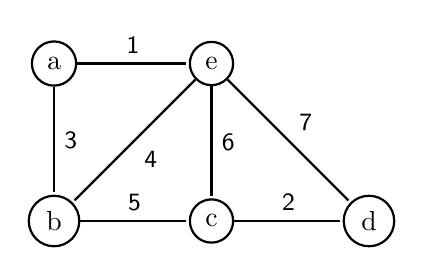
\begin{tikzpicture}[>=stealth',shorten >=1pt,auto,node distance=2cm,
	thick,main node/.style={circle,draw}]
	
	\node[main node] (a) {a};
	\node[main node] (e) [right of=a] {e};
	\node[main node] (b) [below of=a] {b};
	\node[main node] (c) [below of=e] {c};
	\node[main node] (d) [right of=c] {d};
	
	\path[every node/.style={font=\sffamily\small}]
	(a) edge node [] {1} (e)
	(a)	edge node [] {3} (b)
	(e)	edge node [] {4} (b)
	(e)	edge node [] {6} (c)
	(e) edge node [] {7} (d)
	(b) edge node [] {5} (c)
	(c) edge node [] {2} (d);
	\end{tikzpicture}
\end{figure}

\subsubsection*{Sort the edges}
\begin{table}[H]
	\centering
	\begin{tabular}{|c |c |c| c| c| c| c |c|}
		\hline
		Edge	&	(a,e)	&	(c,d)	&	(a,b)	&	(b,e)	&	(b,c)	&	(e,c)	&	(e,d)\\
		\hline
		Weight	&	1		&	2		&	3		&	4		&	5		&	6		&	7\\
		\hline
	\end{tabular}
\end{table}

\subsubsection*{Initial Graph}

\begin{figure}[H]
	\centering
	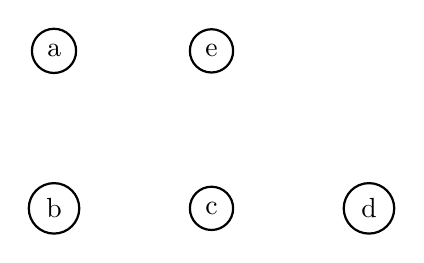
\begin{tikzpicture}[>=stealth',shorten >=1pt,auto,node distance=2cm,
	thick,main node/.style={circle,draw}]
	
	\node[main node] (a) {a};
	\node[main node] (e) [right of=a] {e};
	\node[main node] (b) [below of=a] {b};
	\node[main node] (c) [below of=e] {c};
	\node[main node] (d) [right of=c] {d};
	\end{tikzpicture}
\end{figure}

\subsubsection*{Adding Edge (a,e)}

\begin{figure}[H]
	\centering
	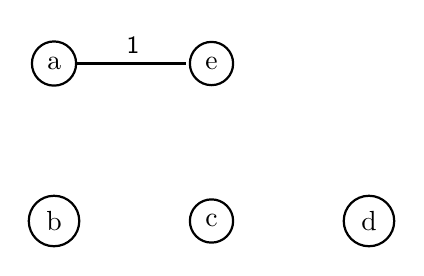
\begin{tikzpicture}[>=stealth',shorten >=1pt,auto,node distance=2cm,
	thick,main node/.style={circle,draw}]
	
	\node[main node] (a) {a};
	\node[main node] (e) [right of=a] {e};
	\node[main node] (b) [below of=a] {b};
	\node[main node] (c) [below of=e] {c};
	\node[main node] (d) [right of=c] {d};
	
	\path[every node/.style={font=\sffamily\small}]
	(a) edge node [] {1} (e);
	\end{tikzpicture}
\end{figure}

\subsubsection*{Adding Edge (c,d)}

\begin{figure}[H]
	\centering
	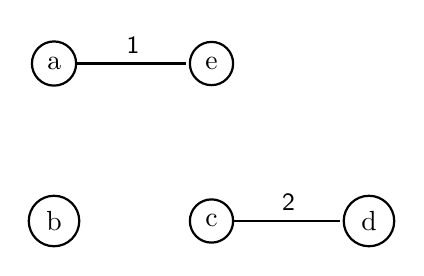
\begin{tikzpicture}[>=stealth',shorten >=1pt,auto,node distance=2cm,
	thick,main node/.style={circle,draw}]
	
	\node[main node] (a) {a};
	\node[main node] (e) [right of=a] {e};
	\node[main node] (b) [below of=a] {b};
	\node[main node] (c) [below of=e] {c};
	\node[main node] (d) [right of=c] {d};
	
	\path[every node/.style={font=\sffamily\small}]
	(a) edge node [] {1} (e)
	(c) edge node [] {2} (d);
	\end{tikzpicture}
\end{figure}

\subsubsection*{Adding Edge (a,b)}

\begin{figure}[H]
	\centering
	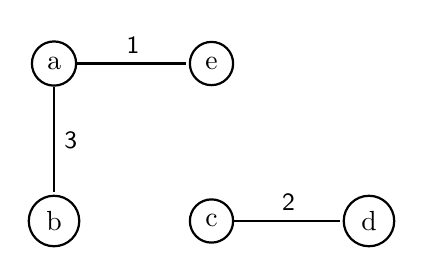
\begin{tikzpicture}[>=stealth',shorten >=1pt,auto,node distance=2cm,
	thick,main node/.style={circle,draw}]
	
	\node[main node] (a) {a};
	\node[main node] (e) [right of=a] {e};
	\node[main node] (b) [below of=a] {b};
	\node[main node] (c) [below of=e] {c};
	\node[main node] (d) [right of=c] {d};
	
	\path[every node/.style={font=\sffamily\small}]
	(a) edge node [] {1} (e)
	(c) edge node [] {2} (d)
	(a) edge node [] {3} (b);
	\end{tikzpicture}
\end{figure}

\subsubsection*{Adding Edge (b,e)}

\begin{figure}[H]
	\centering
	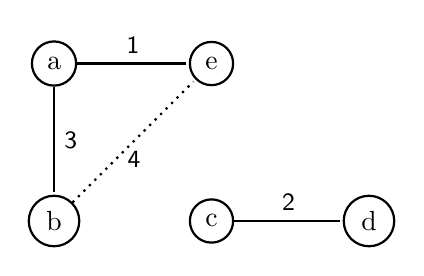
\begin{tikzpicture}[>=stealth',shorten >=1pt,auto,node distance=2cm,
	thick,main node/.style={circle,draw}]
	
	\node[main node] (a) {a};
	\node[main node] (e) [right of=a] {e};
	\node[main node] (b) [below of=a] {b};
	\node[main node] (c) [below of=e] {c};
	\node[main node] (d) [right of=c] {d};
	
	\path[every node/.style={font=\sffamily\small}]
	(a) edge node [] {1} (e)
	(c) edge node [] {2} (d)
	(a) edge node [] {3} (b)
	(b)	edge [dotted] node [below] {4} (e);
	\end{tikzpicture}
	\caption*{Cannot add this edge since it vertex b and vertex e are already in the same tree. }
\end{figure}

\subsubsection*{Adding Edge (b,c)}

\begin{figure}[H]
	\centering
	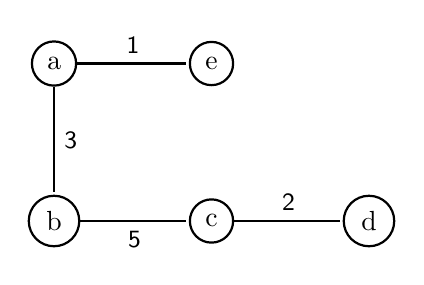
\begin{tikzpicture}[>=stealth',shorten >=1pt,auto,node distance=2cm,
	thick,main node/.style={circle,draw}]
	
	\node[main node] (a) {a};
	\node[main node] (e) [right of=a] {e};
	\node[main node] (b) [below of=a] {b};
	\node[main node] (c) [below of=e] {c};
	\node[main node] (d) [right of=c] {d};
	
	\path[every node/.style={font=\sffamily\small}]
	(a) edge node [] {1} (e)
	(c) edge node [] {2} (d)
	(a) edge node [] {3} (b)
	(b)	edge [] node [below] {5} (c);
	\end{tikzpicture}
	\caption*{All vertices in same tree. Therefore, minimum spanning tree has been derived.}
\end{figure}

\newpage

\section{Minimum Spanning Tree: Prim's Algorithm}

\subsection*{Steps}
\begin{enumerate}
	\item Define an empty tree. 
	\item Select an arbitrary vertex to add to the tree.
	\item Add the least weight edge that connects to the tree.
	\item Repeat until all vertices are connected.
\end{enumerate}

\subsection*{Complexity}
$$
\text{Using adjacency matrix: } O(\vert V \vert^2 )
$$
$$
\text{Using binary heap and adjacency list: } O((\vert V \vert + \vert E \vert) \log(\vert V \vert)) = O(\vert E \vert \log(\vert V \vert))
$$
$$
\text{Using Fibonacci heap and adjacency list: } O(\vert E \vert + \vert V \vert \log(\vert V \vert))
$$

\subsection{Example}
\textbf{Find the minimum spanning tree of the following graph using Prim's algorithm.}

\begin{figure}[H]
	\centering
	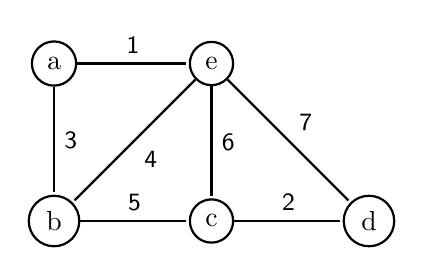
\begin{tikzpicture}[>=stealth',shorten >=1pt,auto,node distance=2cm,
	thick,main node/.style={circle,draw}]
	
	\node[main node] (a) {a};
	\node[main node] (e) [right of=a] {e};
	\node[main node] (b) [below of=a] {b};
	\node[main node] (c) [below of=e] {c};
	\node[main node] (d) [right of=c] {d};
	
	\path[every node/.style={font=\sffamily\small}]
	(a) edge node [] {1} (e)
	(a)	edge node [] {3} (b)
	(e)	edge node [] {4} (b)
	(e)	edge node [] {6} (c)
	(e) edge node [] {7} (d)
	(b) edge node [] {5} (c)
	(c) edge node [] {2} (d);
	\end{tikzpicture}
\end{figure}

\subsubsection*{Initial Tree Starting from Vertex a}

\begin{figure}[H]
	\centering
	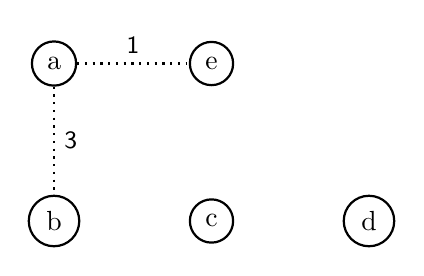
\begin{tikzpicture}[>=stealth',shorten >=1pt,auto,node distance=2cm,
	thick,main node/.style={circle,draw}]
	
	\node[main node] (a) {a};
	\node[main node] (e) [right of=a] {e};
	\node[main node] (b) [below of=a] {b};
	\node[main node] (c) [below of=e] {c};
	\node[main node] (d) [right of=c] {d};
	
	\path[every node/.style={font=\sffamily\small}]
	(a) edge [dotted] node [] {1} (e)
	(a) edge [dotted] node [] {3} (b);
	\end{tikzpicture}
\end{figure}

\subsubsection*{Add edge (a,e)}

\begin{figure}[H]
	\centering
	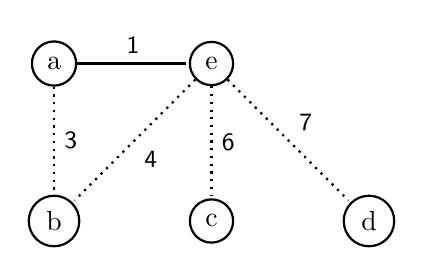
\begin{tikzpicture}[>=stealth',shorten >=1pt,auto,node distance=2cm,
	thick,main node/.style={circle,draw}]
	
	\node[main node] (a) {a};
	\node[main node] (e) [right of=a] {e};
	\node[main node] (b) [below of=a] {b};
	\node[main node] (c) [below of=e] {c};
	\node[main node] (d) [right of=c] {d};
	
	\path[every node/.style={font=\sffamily\small}]
	(a) edge node [] {1} (e)
	(a)	edge [dotted] node [] {3} (b)
	(e)	edge [dotted] node [] {4} (b)
	(e)	edge [dotted] node [] {6} (c)
	(e) edge [dotted] node [] {7} (d);
	\end{tikzpicture}
\end{figure}

\subsubsection*{Add edge (a,b)}

\begin{figure}[H]
	\centering
	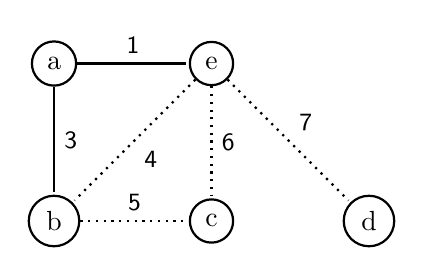
\begin{tikzpicture}[>=stealth',shorten >=1pt,auto,node distance=2cm,
	thick,main node/.style={circle,draw}]
	
	\node[main node] (a) {a};
	\node[main node] (e) [right of=a] {e};
	\node[main node] (b) [below of=a] {b};
	\node[main node] (c) [below of=e] {c};
	\node[main node] (d) [right of=c] {d};
	
	\path[every node/.style={font=\sffamily\small}]
	(a) edge node [] {1} (e)
	(a)	edge [] node [] {3} (b)
	(e)	edge [dotted] node [] {4} (b)
	(e)	edge [dotted] node [] {6} (c)
	(e) edge [dotted] node [] {7} (d)
	(b) edge [dotted] node [] {5} (c);
	\end{tikzpicture}
\end{figure}

\subsubsection*{Add edge (a,b)}

\begin{figure}[H]
	\centering
	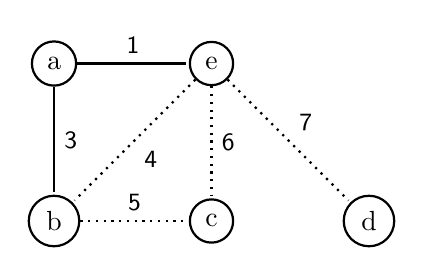
\begin{tikzpicture}[>=stealth',shorten >=1pt,auto,node distance=2cm,
	thick,main node/.style={circle,draw}]
	
	\node[main node] (a) {a};
	\node[main node] (e) [right of=a] {e};
	\node[main node] (b) [below of=a] {b};
	\node[main node] (c) [below of=e] {c};
	\node[main node] (d) [right of=c] {d};
	
	\path[every node/.style={font=\sffamily\small}]
	(a) edge node [] {1} (e)
	(a)	edge [] node [] {3} (b)
	(e)	edge [dotted] node [] {4} (b)
	(e)	edge [dotted] node [] {6} (c)
	(b) edge [dotted] node [] {5} (c)
	(e) edge [dotted] node [] {7} (d);
	\end{tikzpicture}
\end{figure}

\subsubsection*{Add edge (b,e)}

\begin{figure}[H]
	\centering
	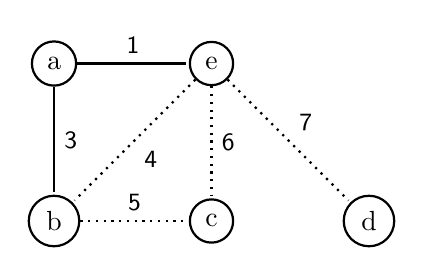
\begin{tikzpicture}[>=stealth',shorten >=1pt,auto,node distance=2cm,
	thick,main node/.style={circle,draw}]
	
	\node[main node] (a) {a};
	\node[main node] (e) [right of=a] {e};
	\node[main node] (b) [below of=a] {b};
	\node[main node] (c) [below of=e] {c};
	\node[main node] (d) [right of=c] {d};
	
	\path[every node/.style={font=\sffamily\small}]
	(a) edge node [] {1} (e)
	(a)	edge [] node [] {3} (b)
	(e)	edge [dotted] node [] {4} (b)
	(e)	edge [dotted] node [] {6} (c)
	(b) edge [dotted] node [] {5} (c)
	(e) edge [dotted] node [] {7} (d);
	\end{tikzpicture}
	\caption*{Cannot edge (b,e) since vertex b and vertex e are in the same tree.}
\end{figure}

\subsubsection*{Add edge (b,c)}

\begin{figure}[H]
	\centering
	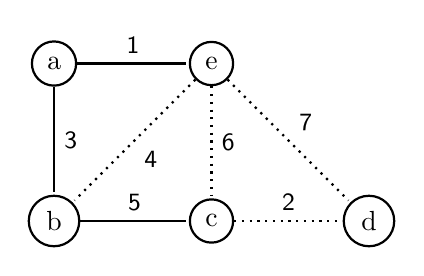
\begin{tikzpicture}[>=stealth',shorten >=1pt,auto,node distance=2cm,
	thick,main node/.style={circle,draw}]
	
	\node[main node] (a) {a};
	\node[main node] (e) [right of=a] {e};
	\node[main node] (b) [below of=a] {b};
	\node[main node] (c) [below of=e] {c};
	\node[main node] (d) [right of=c] {d};
	
	\path[every node/.style={font=\sffamily\small}]
	(a) edge node [] {1} (e)
	(a)	edge [] node [] {3} (b)
	(e)	edge [dotted] node [] {4} (b)
	(e)	edge [dotted] node [] {6} (c)
	(b) edge [] node [] {5} (c)
	(e) edge [dotted] node [] {7} (d)
	(c) edge [dotted] node [] {2} (d);
	\end{tikzpicture}
\end{figure}

\subsubsection*{Add edge (c,d)}

\begin{figure}[H]
	\centering
	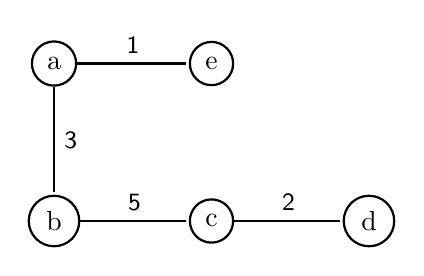
\begin{tikzpicture}[>=stealth',shorten >=1pt,auto,node distance=2cm,
	thick,main node/.style={circle,draw}]
	
	\node[main node] (a) {a};
	\node[main node] (e) [right of=a] {e};
	\node[main node] (b) [below of=a] {b};
	\node[main node] (c) [below of=e] {c};
	\node[main node] (d) [right of=c] {d};
	
	\path[every node/.style={font=\sffamily\small}]
	(a) edge node [] {1} (e)
	(a)	edge [] node [] {3} (b)
	(b) edge [] node [] {5} (c)
	(c) edge [] node [] {2} (d);
	\end{tikzpicture}
	\caption*{All vertices in same tree. Therefore, minimum spanning tree has been derived.}
\end{figure}
\newpage

\section{Breadth-First Search (BFS)}

\subsection*{Problem Statement}
Given a graph $G$ and a vertex $v \in Graph$, find all vertices reachable from $v$ as they are discovered.

\subsection*{Pseudocode}
\begin{algorithm}
	\begin{algorithmic}[1]
		\Procedure{Breadth-First-Search}{G,v}
		\State Let Q be defined as a queue
		\State Q.enqueue(v)\\
		\State v.discovered = true\\
		\While{Q is not empty}
			\State u = Q.dequeue()
			\State (Arbitrary Processing of Node u)
			\For{Edge $e \in E$ where $ e = (u,w)$}
				\If{w.discovered $!=$ true}
					\State Q.enqueue(w);
					\State w.discovered = true
				\EndIf
			\EndFor
		\EndWhile
		\EndProcedure
	\end{algorithmic}
\end{algorithm}

\subsection*{Steps}
\begin{enumerate}
	\item Assume there exists some queue Q.
	\item Starting from a given vertex $v$, mark $v$ as discovered and enqueue $v$ into the Q.
	\item For every iteration:
	\begin{enumerate}
		\item Dequeue the next vertex in Q and define this dequeued vertex as $u$.
		\item For every vertex $w$ that is connected to vertex $u$ by some edge, enqueue each of them in lexical order (alphabetical order) and mark them as discovered.
		\item Repeat until Q is empty.
	\end{enumerate}
\end{enumerate}

\subsection*{Complexity}
$$
O(\vert V \vert + \vert E \vert)
$$

\newpage

\subsection{Example}
\textbf{Given the following graph $G$, perform a breadth-first search from vertex $a$ and print the order that vertices are discovered.}
\begin{figure}[H]
	\centering
	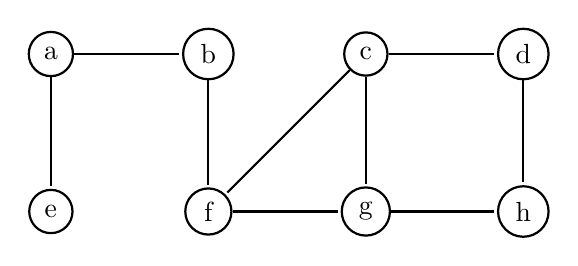
\begin{tikzpicture}[>=stealth',shorten >=1pt,auto,node distance=2cm,
	thick,main node/.style={circle,draw}]
	
	\node[main node] (a) {a};
	\node[main node] (b) [right of=a] {b};
	\node[main node] (c) [right of=b] {c};
	\node[main node] (d) [right of=c] {d};
	\node[main node] (e) [below of=a] {e};
	\node[main node] (f) [below of=b] {f};
	\node[main node] (g) [below of=c] {g};
	\node[main node] (h) [below of=d] {h};
		
	\path[every node/.style={font=\sffamily\small}]
	(a) edge node [] {} (b)
	(a)	edge node [] {} (e)
	(b)	edge node [] {} (f)
	(c)	edge node [] {} (d)
	(c)	edge node [] {} (f)
	(c)	edge node [] {} (g)
	(d) edge node [] {} (h)
	(f) edge node [] {} (g)
	(g) edge node [] {} (h);
	\end{tikzpicture}
\end{figure}

\subsubsection*{Initialization}
$$
Q = \{ a \}
$$
\begin{figure}[H]
	\centering
	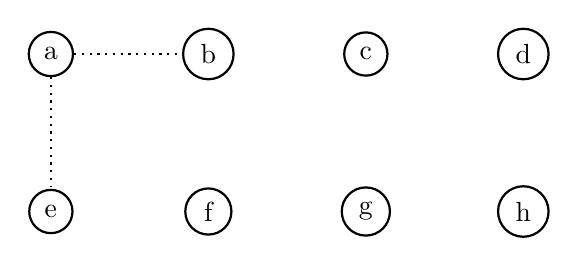
\begin{tikzpicture}[>=stealth',shorten >=1pt,auto,node distance=2cm,
	thick,main node/.style={circle,draw}]
	
	\node[main node] (a) {a};
	\node[main node] (b) [right of=a] {b};
	\node[main node] (c) [right of=b] {c};
	\node[main node] (d) [right of=c] {d};
	\node[main node] (e) [below of=a] {e};
	\node[main node] (f) [below of=b] {f};
	\node[main node] (g) [below of=c] {g};
	\node[main node] (h) [below of=d] {h};
	
	\path[every node/.style={font=\sffamily\small}]
	(a) edge [dotted] node [] {} (b)
	(a)	edge [dotted] node [] {} (e);
	\end{tikzpicture}
\end{figure}

\subsubsection*{Dequeue a and Enqueue b,e}
$$
Q = \{ b,e \}
$$
\begin{figure}[H]
	\centering
	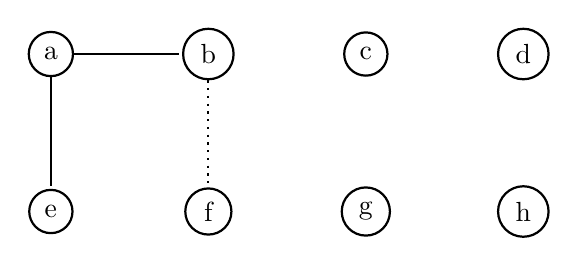
\begin{tikzpicture}[>=stealth',shorten >=1pt,auto,node distance=2cm,
	thick,main node/.style={circle,draw}]
	
	\node[main node] (a) {a};
	\node[main node] (b) [right of=a] {b};
	\node[main node] (c) [right of=b] {c};
	\node[main node] (d) [right of=c] {d};
	\node[main node] (e) [below of=a] {e};
	\node[main node] (f) [below of=b] {f};
	\node[main node] (g) [below of=c] {g};
	\node[main node] (h) [below of=d] {h};
	
	\path[every node/.style={font=\sffamily\small}]
	(a) edge [] node [] {} (b)
	(a)	edge [] node [] {} (e)
	(b)	edge [dotted] node [] {} (f);
	\end{tikzpicture}
\end{figure}
$$
\text{Order of Discovery: } a
$$

\subsubsection*{Dequeue b and Enqueue f}
$$
Q = \{ e, f \}
$$
\begin{figure}[H]
	\centering
	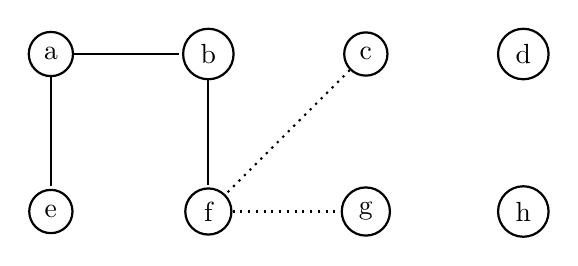
\begin{tikzpicture}[>=stealth',shorten >=1pt,auto,node distance=2cm,
	thick,main node/.style={circle,draw}]
	
	\node[main node] (a) {a};
	\node[main node] (b) [right of=a] {b};
	\node[main node] (c) [right of=b] {c};
	\node[main node] (d) [right of=c] {d};
	\node[main node] (e) [below of=a] {e};
	\node[main node] (f) [below of=b] {f};
	\node[main node] (g) [below of=c] {g};
	\node[main node] (h) [below of=d] {h};
	
	\path[every node/.style={font=\sffamily\small}]
	(a) edge [] node [] {} (b)
	(a)	edge [] node [] {} (e)
	(b)	edge [] node [] {} (f)
	(c)	edge [dotted] node [] {} (f)
	(f) edge [dotted] node [] {} (g);
	\end{tikzpicture}
\end{figure}
$$
\text{Order of Discovery: } a, b
$$

\subsubsection*{Dequeue e and Enqueue Nothing}
$$
Q = \{ f \}
$$
\begin{figure}[H]
	\centering
	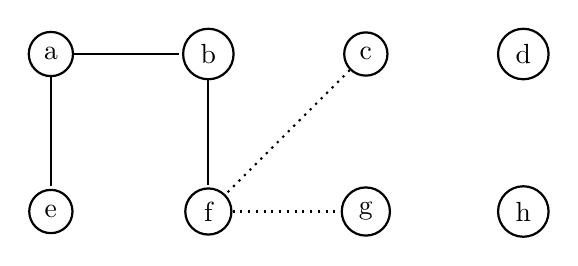
\begin{tikzpicture}[>=stealth',shorten >=1pt,auto,node distance=2cm,
	thick,main node/.style={circle,draw}]
	
	\node[main node] (a) {a};
	\node[main node] (b) [right of=a] {b};
	\node[main node] (c) [right of=b] {c};
	\node[main node] (d) [right of=c] {d};
	\node[main node] (e) [below of=a] {e};
	\node[main node] (f) [below of=b] {f};
	\node[main node] (g) [below of=c] {g};
	\node[main node] (h) [below of=d] {h};
	
	\path[every node/.style={font=\sffamily\small}]
	(a) edge [] node [] {} (b)
	(a)	edge [] node [] {} (e)
	(b)	edge [] node [] {} (f)
	(c)	edge [dotted] node [] {} (f)
	(f) edge [dotted] node [] {} (g);
	\end{tikzpicture}
\end{figure}
$$
\text{Order of Discovery: } a, b, e
$$

\subsubsection*{Dequeue f and Enqueue c,g}
$$
Q = \{ c,g  \}
$$
\begin{figure}[H]
	\centering
	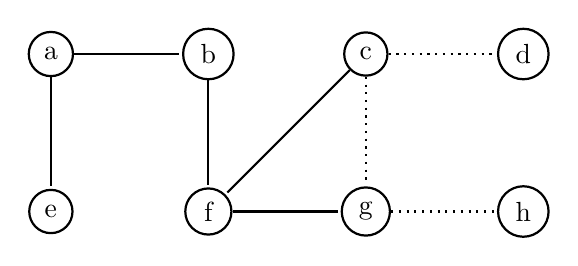
\begin{tikzpicture}[>=stealth',shorten >=1pt,auto,node distance=2cm,
	thick,main node/.style={circle,draw}]
	
	\node[main node] (a) {a};
	\node[main node] (b) [right of=a] {b};
	\node[main node] (c) [right of=b] {c};
	\node[main node] (d) [right of=c] {d};
	\node[main node] (e) [below of=a] {e};
	\node[main node] (f) [below of=b] {f};
	\node[main node] (g) [below of=c] {g};
	\node[main node] (h) [below of=d] {h};
	
	\path[every node/.style={font=\sffamily\small}]
	(a) edge [] node [] {} (b)
	(a)	edge [] node [] {} (e)
	(b)	edge [] node [] {} (f)
	(c)	edge [dotted] node [] {} (d)
	(c)	edge [] node [] {} (f)
	(c) edge [dotted] node[] {} (g)
	(f) edge node [] {} (g)
	(g) edge [dotted] node [] {} (h);
	\end{tikzpicture}
\end{figure}
$$
\text{Order of Discovery: } a, b, e, f
$$

\subsubsection*{Dequeue c and Enqueue d}
$$
Q = \{ g, d  \}
$$
\begin{figure}[H]
	\centering
	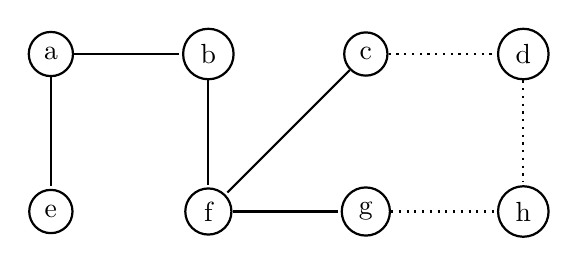
\begin{tikzpicture}[>=stealth',shorten >=1pt,auto,node distance=2cm,
	thick,main node/.style={circle,draw}]
	
	\node[main node] (a) {a};
	\node[main node] (b) [right of=a] {b};
	\node[main node] (c) [right of=b] {c};
	\node[main node] (d) [right of=c] {d};
	\node[main node] (e) [below of=a] {e};
	\node[main node] (f) [below of=b] {f};
	\node[main node] (g) [below of=c] {g};
	\node[main node] (h) [below of=d] {h};
	
	\path[every node/.style={font=\sffamily\small}]
	(a) edge [] node [] {} (b)
	(a)	edge [] node [] {} (e)
	(b)	edge [] node [] {} (f)
	(c)	edge [dotted] node [] {} (d)
	(c)	edge [] node [] {} (f)
	(d) edge [dotted] node [] {} (h)
	(f) edge node [] {} (g)
	(g) edge [dotted] node [] {} (h);
	\end{tikzpicture}
	\caption*{Note that when c is processed, it notices that g is already discovered so it does not attempt that edge. Hence why the dotted edge (c,g) disappears.}
\end{figure}
$$
\text{Order of Discovery: } a, b, e, f, c
$$

\newpage

\subsubsection*{Dequeue g and Enqueue h}
$$
Q = \{ d, h  \}
$$
\begin{figure}[H]
	\centering
	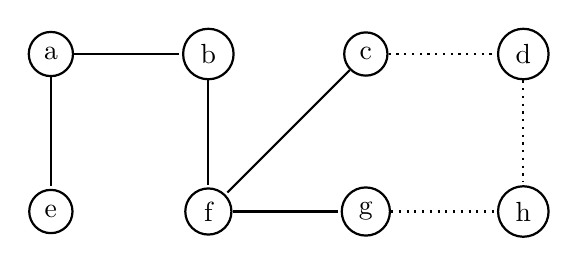
\begin{tikzpicture}[>=stealth',shorten >=1pt,auto,node distance=2cm,
	thick,main node/.style={circle,draw}]
	
	\node[main node] (a) {a};
	\node[main node] (b) [right of=a] {b};
	\node[main node] (c) [right of=b] {c};
	\node[main node] (d) [right of=c] {d};
	\node[main node] (e) [below of=a] {e};
	\node[main node] (f) [below of=b] {f};
	\node[main node] (g) [below of=c] {g};
	\node[main node] (h) [below of=d] {h};
	
	\path[every node/.style={font=\sffamily\small}]
	(a) edge [] node [] {} (b)
	(a)	edge [] node [] {} (e)
	(b)	edge [] node [] {} (f)
	(c)	edge [dotted] node [] {} (d)
	(c)	edge [] node [] {} (f)
	(d) edge [dotted] node [] {} (h)
	(f) edge node [] {} (g)
	(g) edge [dotted] node [] {} (h);
	\end{tikzpicture}
\end{figure}
$$
\text{Order of Discovery: } a, b, e, f, c, g
$$

\subsubsection*{Dequeue d and Enqueue Nothing}
$$
Q = \{ d, h  \}
$$
\begin{figure}[H]
	\centering
	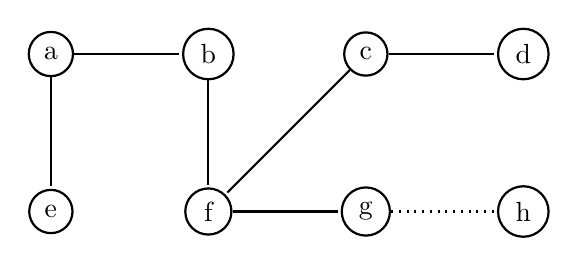
\begin{tikzpicture}[>=stealth',shorten >=1pt,auto,node distance=2cm,
	thick,main node/.style={circle,draw}]
	
	\node[main node] (a) {a};
	\node[main node] (b) [right of=a] {b};
	\node[main node] (c) [right of=b] {c};
	\node[main node] (d) [right of=c] {d};
	\node[main node] (e) [below of=a] {e};
	\node[main node] (f) [below of=b] {f};
	\node[main node] (g) [below of=c] {g};
	\node[main node] (h) [below of=d] {h};
	
	\path[every node/.style={font=\sffamily\small}]
	(a) edge [] node [] {} (b)
	(a)	edge [] node [] {} (e)
	(b)	edge [] node [] {} (f)
	(c)	edge [] node [] {} (d)
	(c)	edge [] node [] {} (f)
	(f) edge node [] {} (g)
	(g) edge [dotted] node [] {} (h);
	\end{tikzpicture}
\end{figure}
$$
\text{Order of Discovery: } a, b, e, f, c, g, d
$$

\subsubsection*{Dequeue h and Enqueue Nothing}
$$
Q = \{ h  \}
$$
\begin{figure}[H]
	\centering
	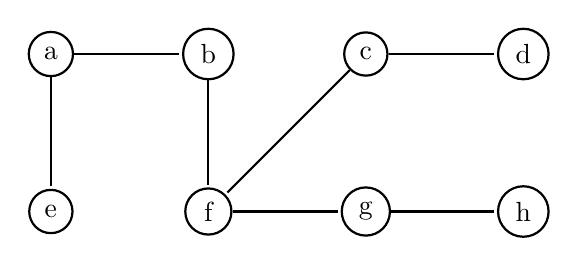
\begin{tikzpicture}[>=stealth',shorten >=1pt,auto,node distance=2cm,
	thick,main node/.style={circle,draw}]
	
	\node[main node] (a) {a};
	\node[main node] (b) [right of=a] {b};
	\node[main node] (c) [right of=b] {c};
	\node[main node] (d) [right of=c] {d};
	\node[main node] (e) [below of=a] {e};
	\node[main node] (f) [below of=b] {f};
	\node[main node] (g) [below of=c] {g};
	\node[main node] (h) [below of=d] {h};
	
	\path[every node/.style={font=\sffamily\small}]
	(a) edge [] node [] {} (b)
	(a)	edge [] node [] {} (e)
	(b)	edge [] node [] {} (f)
	(c)	edge [] node [] {} (d)
	(c)	edge [] node [] {} (f)
	(f) edge node [] {} (g)
	(g) edge [] node [] {} (h);
	\end{tikzpicture}
\end{figure}
$$
\text{Order of Discovery: } a, b, e, f, c, g, d, h
$$
\newpage

\section{Case Study: Depth-First Search (DFS)}

\subsection{Definitions}
\begin{itemize}
	\item \textbf{Tree Edge: } Edge in the depth-first forest $G_\pi$ where $v$ was first discovered by exploring edge $(u,v)$.
	\item \textbf{Back Edge: } Edge $(u,v)$ connecting vertex $u$ to an ancestor $v$.
	\item \textbf{Forward Edge: } Nontree edge $(u,v)$ connecting vertex $u$ to a descendant $v$.
	\item \textbf{Cross Edge: } Any other edge that does not fall in the category of the previous three.
\end{itemize}

\subsection*{Steps}
\begin{enumerate}
	\item All vertices are defined to have a discovery time, finish time, and a color that defines its state.
	\item Define a timer $t$ that tracks the number of operations we've performed (visit an edge or finish processing an edge). 
	\item Given a starting vertex $v$, visit that vertex.
	\item Visiting a given vertex $u$:
	\begin{enumerate}
		\item Increase the timer by 1 and the start time of vertex $u$ is the value of the timer.
		\item The color of vertex $u$ is then set to GRAY for visited, but not finished.
		\item For every vertex that $u$ is connected to and has the color WHITE, visit those vertices in lexical order.
		\item Once all vertices that $u$ is connected to have been visited and finished, the color of $u$ is set to BLACK for finished.
		\item The timer is increased by 1 again and the finish time of vertex $u$ is the value of the timer.
	\end{enumerate}
	\item Repeat the visiting vertices until all vertices are finished.
\end{enumerate}

\subsection*{Complexity}
$$
\Theta(\vert V \vert + \vert E \vert)
$$

\newpage

\subsection{Example}
\textbf{Given the following graph $G$, perform a depth-first search from vertex $a$ and print the order that vertices are discovered and label the edges according to their classification.}
\begin{figure}[H]
	\centering
	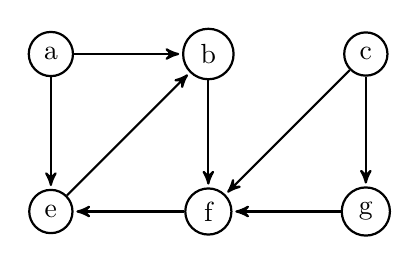
\begin{tikzpicture}[->,>=stealth',shorten >=1pt,auto,node distance=2cm,
	thick,main node/.style={circle,draw}]
	
	\definecolor{gray}{RGB}{200,200,200}
	
	\node[main node] (a) {a};
	\node[main node] (b) [right of=a] {b};
	\node[main node] (c) [right of=b] {c};
	\node[main node] (e) [below of=a] {e};
	\node[main node] (f) [below of=b] {f};
	\node[main node] (g) [below of=c] {g};
	
	\path[every node/.style={font=\sffamily\small}]
	(a) edge node [] {} (b)
	(a)	edge node [] {} (e)
	(b)	edge node [] {} (f)
	(c)	edge node [] {} (f)
	(c)	edge node [] {} (g)
	(e) edge node [] {} (b)
	(f) edge node [] {} (e)
	(g)	edge node [] {} (f);
	\end{tikzpicture}
\end{figure}

\subsubsection*{Visit Vertex a (Given)}

\begin{figure}[H]
	\centering
	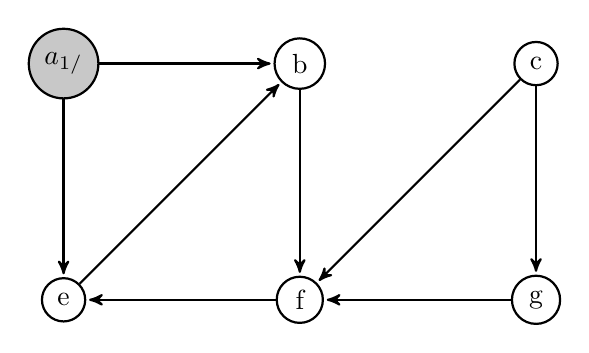
\begin{tikzpicture}[->,>=stealth',shorten >=1pt,auto,node distance=3cm,
	thick,main node/.style={circle,draw}]
	
	\definecolor{gray}{RGB}{200,200,200}
	
	\node[main node, fill=gray] (a) {$a_{1/}$};
	\node[main node] (b) [right of=a] {b};
	\node[main node] (c) [right of=b] {c};
	\node[main node] (e) [below of=a] {e};
	\node[main node] (f) [below of=b] {f};
	\node[main node] (g) [below of=c] {g};
	
	\path[every node/.style={font=\sffamily\small}]
	(a) edge node [] {} (b)
	(a)	edge node [] {} (e)
	(b)	edge node [] {} (f)
	(c)	edge node [] {} (f)
	(c)	edge node [] {} (g)
	(e) edge node [] {} (b)
	(f) edge node [] {} (e)
	(g)	edge node [] {} (f);
	\end{tikzpicture}
\end{figure}

\subsubsection*{Visit Vertex b from Vertex a}

\begin{figure}[H]
	\centering
	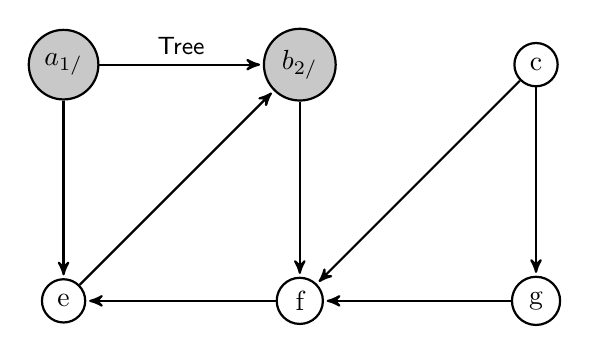
\begin{tikzpicture}[->,>=stealth',shorten >=1pt,auto,node distance=3cm,
	thick,main node/.style={circle,draw}]
	
	\definecolor{gray}{RGB}{200,200,200}
	
	\node[main node, fill=gray] (a) {$a_{1/}$};
	\node[main node, fill=gray] (b) [right of=a] {$b_{2/}$};
	\node[main node] (c) [right of=b] {c};
	\node[main node] (e) [below of=a] {e};
	\node[main node] (f) [below of=b] {f};
	\node[main node] (g) [below of=c] {g};
	
	\path[every node/.style={font=\sffamily\small}]
	(a) edge node [] {Tree} (b)
	(a)	edge node [] {} (e)
	(b)	edge node [] {} (f)
	(c)	edge node [] {} (f)
	(c)	edge node [] {} (g)
	(e) edge node [] {} (b)
	(f) edge node [] {} (e)
	(g)	edge node [] {} (f);
	\end{tikzpicture}
\end{figure}

\subsubsection*{Visit Vertex f from Vertex b}

\begin{figure}[H]
	\centering
	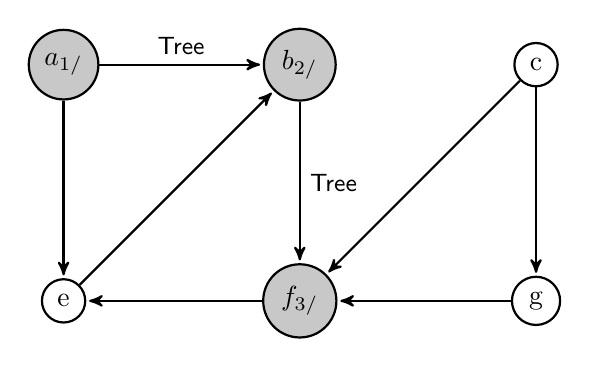
\begin{tikzpicture}[->,>=stealth',shorten >=1pt,auto,node distance=3cm,
	thick,main node/.style={circle,draw}]
	
	\definecolor{gray}{RGB}{200,200,200}
	
	\node[main node, fill=gray] (a) {$a_{1/}$};
	\node[main node, fill=gray] (b) [right of=a] {$b_{2/}$};
	\node[main node] (c) [right of=b] {c};
	\node[main node] (e) [below of=a] {e};
	\node[main node, fill=gray] (f) [below of=b] {$f_{3/}$};
	\node[main node] (g) [below of=c] {g};
	
	\path[every node/.style={font=\sffamily\small}]
	(a) edge node [] {Tree} (b)
	(a)	edge node [] {} (e)
	(b)	edge node [] {Tree} (f)
	(c)	edge node [] {} (f)
	(c)	edge node [] {} (g)
	(e) edge node [] {} (b)
	(f) edge node [] {} (e)
	(g)	edge node [] {} (f);
	\end{tikzpicture}
\end{figure}

\subsubsection*{Visit Vertex e from Vertex f}

\begin{figure}[H]
	\centering
	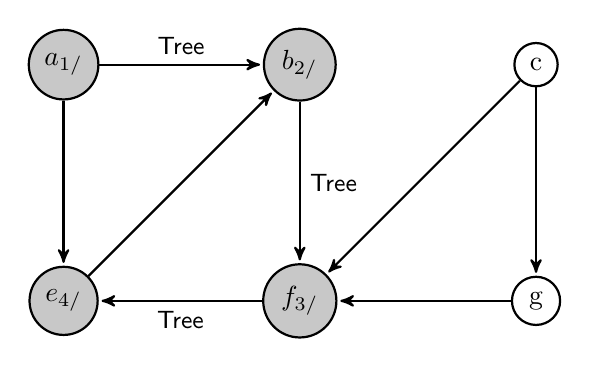
\begin{tikzpicture}[->,>=stealth',shorten >=1pt,auto,node distance=3cm,
	thick,main node/.style={circle,draw}]
	
	\definecolor{gray}{RGB}{200,200,200}
	
	\node[main node, fill=gray] (a) {$a_{1/}$};
	\node[main node, fill=gray] (b) [right of=a] {$b_{2/}$};
	\node[main node] (c) [right of=b] {c};
	\node[main node,fill=gray] (e) [below of=a] {$e_{4/}$};
	\node[main node, fill=gray] (f) [below of=b] {$f_{3/}$};
	\node[main node] (g) [below of=c] {g};
	
	\path[every node/.style={font=\sffamily\small}]
	(a) edge node [] {Tree} (b)
	(a)	edge node [] {} (e)
	(b)	edge node [] {Tree} (f)
	(c)	edge node [] {} (f)
	(c)	edge node [] {} (g)
	(e) edge node [] {} (b)
	(f) edge node [] {Tree} (e)
	(g)	edge node [] {} (f);
	\end{tikzpicture}
\end{figure}

\subsubsection*{Attempt to Visit Vertex b from Vertex e and Finishing Vertex e}

\begin{figure}[H]
	\centering
	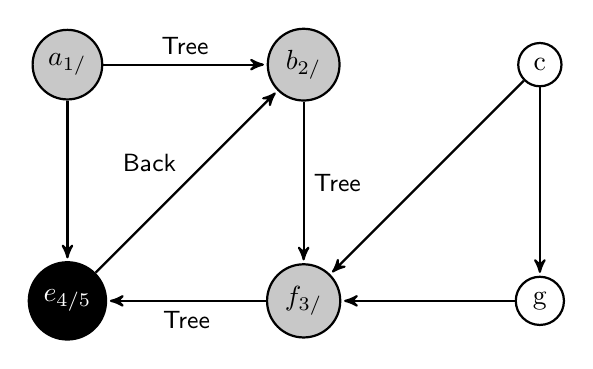
\begin{tikzpicture}[->,>=stealth',shorten >=1pt,auto,node distance=3cm,
	thick,main node/.style={circle,draw}]
	
	\definecolor{gray}{RGB}{200,200,200}
	\definecolor{black}{RGB}{0,0,0}
	
	\node[main node, fill=gray] (a) {$a_{1/}$};
	\node[main node, fill=gray] (b) [right of=a] {$b_{2/}$};
	\node[main node] (c) [right of=b] {c};
	\node[main node,fill=black,text=white] (e) [below of=a] {$e_{4/5}$};
	\node[main node, fill=gray] (f) [below of=b] {$f_{3/}$};
	\node[main node] (g) [below of=c] {g};
	
	\path[every node/.style={font=\sffamily\small}]
	(a) edge node [] {Tree} (b)
	(a)	edge node [] {} (e)
	(b)	edge node [] {Tree} (f)
	(c)	edge node [] {} (f)
	(c)	edge node [] {} (g)
	(e) edge node [] {Back} (b)
	(f) edge node [] {Tree} (e)
	(g)	edge node [] {} (f);
	\end{tikzpicture}
	\caption*{Unable to visit vertex b from vertex e since b does not have the color WHITE. Since attempting to visit from GRAY-colored vertex to another GRAY-colored vertex, this implies that vertex b must be an ancestor of vertex e. Therefore, this edge is a back edge.}
\end{figure}

\subsubsection*{Finishing Vertex f}

\begin{figure}[H]
	\centering
	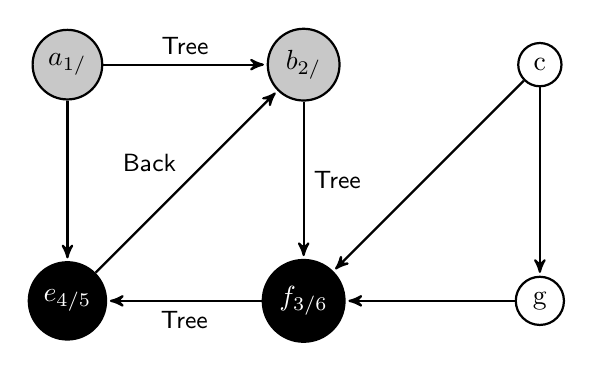
\begin{tikzpicture}[->,>=stealth',shorten >=1pt,auto,node distance=3cm,
	thick,main node/.style={circle,draw}]
	
	\definecolor{gray}{RGB}{200,200,200}
	\definecolor{black}{RGB}{0,0,0}
	
	\node[main node, fill=gray] (a) {$a_{1/}$};
	\node[main node, fill=gray] (b) [right of=a] {$b_{2/}$};
	\node[main node] (c) [right of=b] {c};
	\node[main node,fill=black,text=white] (e) [below of=a] {$e_{4/5}$};
	\node[main node, fill=black, text=white] (f) [below of=b] {$f_{3/6}$};
	\node[main node] (g) [below of=c] {g};
	
	\path[every node/.style={font=\sffamily\small}]
	(a) edge node [] {Tree} (b)
	(a)	edge node [] {} (e)
	(b)	edge node [] {Tree} (f)
	(c)	edge node [] {} (f)
	(c)	edge node [] {} (g)
	(e) edge node [] {Back} (b)
	(f) edge node [] {Tree} (e)
	(g)	edge node [] {} (f);
	\end{tikzpicture}
\end{figure}

\subsubsection*{Finishing Vertex b}

\begin{figure}[H]
	\centering
	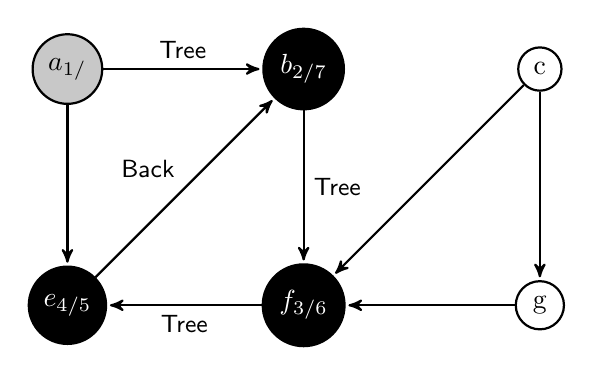
\begin{tikzpicture}[->,>=stealth',shorten >=1pt,auto,node distance=3cm,
	thick,main node/.style={circle,draw}]
	
	\definecolor{gray}{RGB}{200,200,200}
	\definecolor{black}{RGB}{0,0,0}
	
	\node[main node, fill=gray] (a) {$a_{1/}$};
	\node[main node, fill=black,text=white] (b) [right of=a] {$b_{2/7}$};
	\node[main node] (c) [right of=b] {c};
	\node[main node,fill=black,text=white] (e) [below of=a] {$e_{4/5}$};
	\node[main node, fill=black, text=white] (f) [below of=b] {$f_{3/6}$};
	\node[main node] (g) [below of=c] {g};
	
	\path[every node/.style={font=\sffamily\small}]
	(a) edge node [] {Tree} (b)
	(a)	edge node [] {} (e)
	(b)	edge node [] {Tree} (f)
	(c)	edge node [] {} (f)
	(c)	edge node [] {} (g)
	(e) edge node [] {Back} (b)
	(f) edge node [] {Tree} (e)
	(g)	edge node [] {} (f);
	\end{tikzpicture}
\end{figure}

\subsubsection*{Attempt to Visit Vertex e from Vertex a and Finishing Vertex a}

\begin{figure}[H]
	\centering
	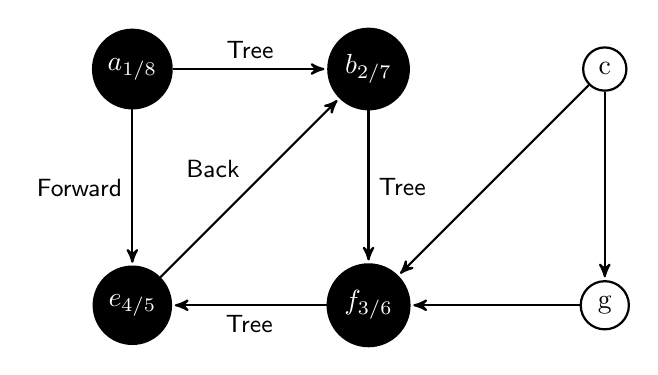
\begin{tikzpicture}[->,>=stealth',shorten >=1pt,auto,node distance=3cm,
	thick,main node/.style={circle,draw}]
	
	\definecolor{gray}{RGB}{200,200,200}
	\definecolor{black}{RGB}{0,0,0}
	
	\node[main node, fill=black,text=white] (a) {$a_{1/8}$};
	\node[main node, fill=black, text=white] (b) [right of=a] {$b_{2/7}$};
	\node[main node] (c) [right of=b] {c};
	\node[main node,fill=black,text=white] (e) [below of=a] {$e_{4/5}$};
	\node[main node, fill=black,text=white] (f) [below of=b] {$f_{3/6}$};
	\node[main node] (g) [below of=c] {g};
	
	\path[every node/.style={font=\sffamily\small}]
	(a) edge node [] {Tree} (b)
	(a)	edge node [left] {Forward} (e)
	(b)	edge node [] {Tree} (f)
	(c)	edge node [] {} (f)
	(c)	edge node [] {} (g)
	(e) edge node [] {Back} (b)
	(f) edge node [] {Tree} (e)
	(g)	edge node [] {} (f);
	\end{tikzpicture}
	\caption*{Unable to visit vertex e from vertex a since vertex e does not have color WHITE. Since attempting to visit a BLACK-colored vertex from a GRAY-colored vertex, it implies that this may be a forward edge or a cross edge. Since we know that vertex e is a descendant of vertex a, this edge must be a forward edge.}
\end{figure}

\subsubsection*{Visit Vertex c}

\begin{figure}[H]
	\centering
	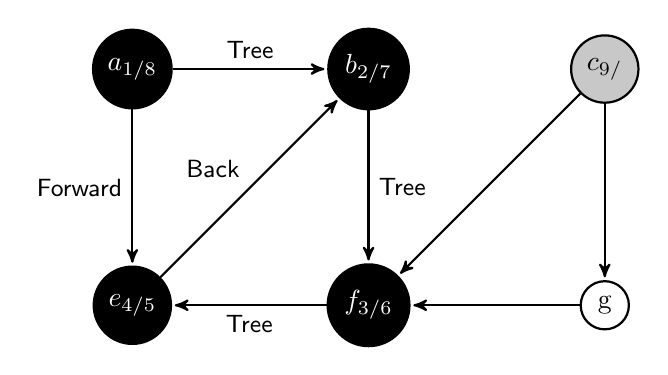
\begin{tikzpicture}[->,>=stealth',shorten >=1pt,auto,node distance=3cm,
	thick,main node/.style={circle,draw}]
	
	\definecolor{gray}{RGB}{200,200,200}
	\definecolor{black}{RGB}{0,0,0}
	
	\node[main node, fill=black,text=white] (a) {$a_{1/8}$};
	\node[main node, fill=black, text=white] (b) [right of=a] {$b_{2/7}$};
	\node[main node, fill=gray] (c) [right of=b] {$c_{9/}$};
	\node[main node,fill=black,text=white] (e) [below of=a] {$e_{4/5}$};
	\node[main node, fill=black,text=white] (f) [below of=b] {$f_{3/6}$};
	\node[main node] (g) [below of=c] {g};
	
	\path[every node/.style={font=\sffamily\small}]
	(a) edge node [] {Tree} (b)
	(a)	edge node [left] {Forward} (e)
	(b)	edge node [] {Tree} (f)
	(c)	edge node [] {} (f)
	(c)	edge node [] {} (g)
	(e) edge node [] {Back} (b)
	(f) edge node [] {Tree} (e)
	(g)	edge node [] {} (f);
	\end{tikzpicture}
	\caption*{Note: Not all vertices have been processed, therefore we choose an unvisited vertex in lexical order.}
\end{figure}

\subsubsection*{Attempt to Visit Vertex f from Vertex c}

\begin{figure}[H]
	\centering
	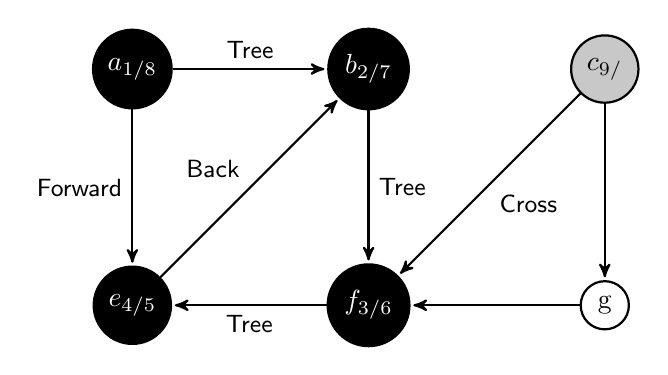
\begin{tikzpicture}[->,>=stealth',shorten >=1pt,auto,node distance=3cm,
	thick,main node/.style={circle,draw}]
	
	\definecolor{gray}{RGB}{200,200,200}
	\definecolor{black}{RGB}{0,0,0}
	
	\node[main node, fill=black,text=white] (a) {$a_{1/8}$};
	\node[main node, fill=black, text=white] (b) [right of=a] {$b_{2/7}$};
	\node[main node, fill=gray] (c) [right of=b] {$c_{9/}$};
	\node[main node,fill=black,text=white] (e) [below of=a] {$e_{4/5}$};
	\node[main node, fill=black,text=white] (f) [below of=b] {$f_{3/6}$};
	\node[main node] (g) [below of=c] {g};
	
	\path[every node/.style={font=\sffamily\small}]
	(a) edge node [] {Tree} (b)
	(a)	edge node [left] {Forward} (e)
	(b)	edge node [] {Tree} (f)
	(c)	edge node [] {Cross} (f)
	(c)	edge node [] {} (g)
	(e) edge node [] {Back} (b)
	(f) edge node [] {Tree} (e)
	(g)	edge node [] {} (f);
	\end{tikzpicture}
	\caption*{Unable to visit vertex f from vertex c since vertex e does not have color WHITE. Since attempting to visit a BLACK-colored vertex from a GRAY-colored vertex, it implies that this may be a forward edge or a cross edge. Since we know that vertex f is not a descendant of vertex c, this edge must be a cross edge.}
\end{figure}

\subsubsection*{Visit Vertex g from Vertex c}

\begin{figure}[H]
	\centering
	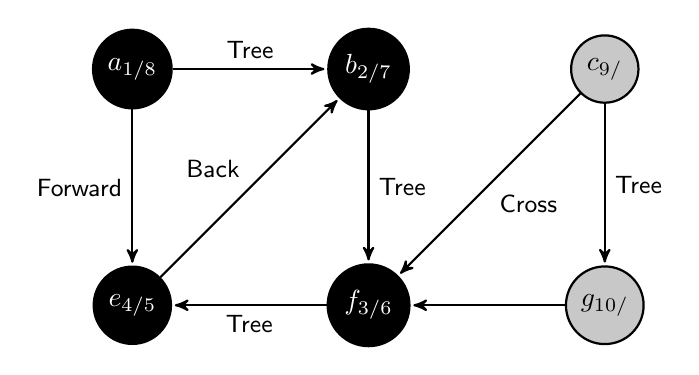
\begin{tikzpicture}[->,>=stealth',shorten >=1pt,auto,node distance=3cm,
	thick,main node/.style={circle,draw}]
	
	\definecolor{gray}{RGB}{200,200,200}
	\definecolor{black}{RGB}{0,0,0}
	
	\node[main node, fill=black,text=white] (a) {$a_{1/8}$};
	\node[main node, fill=black, text=white] (b) [right of=a] {$b_{2/7}$};
	\node[main node, fill=gray] (c) [right of=b] {$c_{9/}$};
	\node[main node,fill=black,text=white] (e) [below of=a] {$e_{4/5}$};
	\node[main node, fill=black,text=white] (f) [below of=b] {$f_{3/6}$};
	\node[main node, fill=gray] (g) [below of=c] {$g_{10/}$};
	
	\path[every node/.style={font=\sffamily\small}]
	(a) edge node [] {Tree} (b)
	(a)	edge node [left] {Forward} (e)
	(b)	edge node [] {Tree} (f)
	(c)	edge node [] {Cross} (f)
	(c)	edge node [] {Tree} (g)
	(e) edge node [] {Back} (b)
	(f) edge node [] {Tree} (e)
	(g)	edge node [] {} (f);
	\end{tikzpicture}
\end{figure}

\subsubsection*{Attempt to Visit Vertex f from Vertex a and Finishing Vertex g}

\begin{figure}[H]
	\centering
	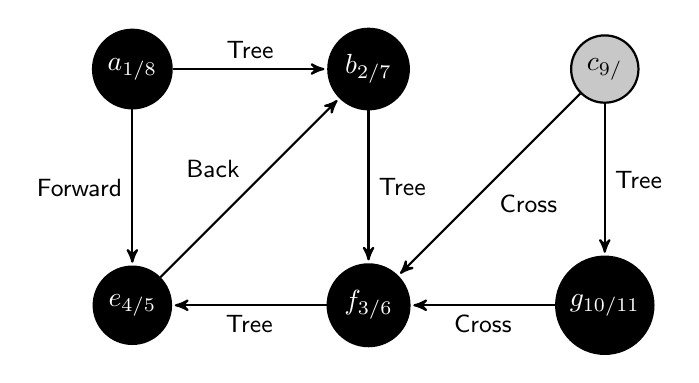
\begin{tikzpicture}[->,>=stealth',shorten >=1pt,auto,node distance=3cm,
	thick,main node/.style={circle,draw}]
	
	\definecolor{gray}{RGB}{200,200,200}
	\definecolor{black}{RGB}{0,0,0}
	
	\node[main node, fill=black,text=white] (a) {$a_{1/8}$};
	\node[main node, fill=black, text=white] (b) [right of=a] {$b_{2/7}$};
	\node[main node, fill=gray] (c) [right of=b] {$c_{9/}$};
	\node[main node,fill=black,text=white] (e) [below of=a] {$e_{4/5}$};
	\node[main node, fill=black,text=white] (f) [below of=b] {$f_{3/6}$};
	\node[main node, fill=black, text=white] (g) [below of=c] {$g_{10/11}$};
	
	\path[every node/.style={font=\sffamily\small}]
	(a) edge node [] {Tree} (b)
	(a)	edge node [left] {Forward} (e)
	(b)	edge node [] {Tree} (f)
	(c)	edge node [] {Cross} (f)
	(c)	edge node [] {Tree} (g)
	(e) edge node [] {Back} (b)
	(f) edge node [] {Tree} (e)
	(g)	edge node [] {Cross} (f);
	\end{tikzpicture}
\end{figure}

\subsubsection*{Finishing Vertex c}

\begin{figure}[H]
	\centering
	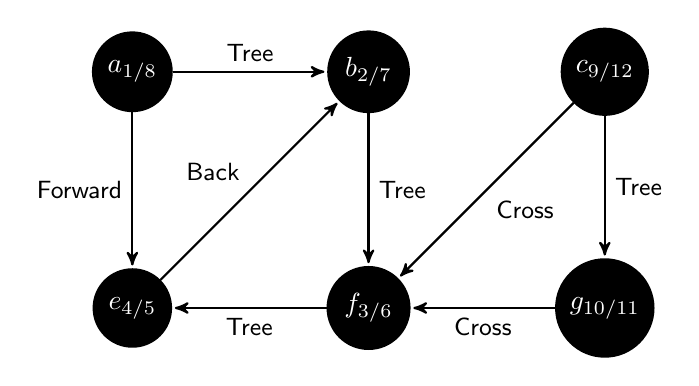
\begin{tikzpicture}[->,>=stealth',shorten >=1pt,auto,node distance=3cm,
	thick,main node/.style={circle,draw}]
	
	\definecolor{gray}{RGB}{200,200,200}
	\definecolor{black}{RGB}{0,0,0}
	
	\node[main node, fill=black,text=white] (a) {$a_{1/8}$};
	\node[main node, fill=black, text=white] (b) [right of=a] {$b_{2/7}$};
	\node[main node, fill=black,text=white] (c) [right of=b] {$c_{9/12}$};
	\node[main node,fill=black,text=white] (e) [below of=a] {$e_{4/5}$};
	\node[main node, fill=black,text=white] (f) [below of=b] {$f_{3/6}$};
	\node[main node, fill=black, text=white] (g) [below of=c] {$g_{10/11}$};
	
	\path[every node/.style={font=\sffamily\small}]
	(a) edge node [] {Tree} (b)
	(a)	edge node [left] {Forward} (e)
	(b)	edge node [] {Tree} (f)
	(c)	edge node [] {Cross} (f)
	(c)	edge node [] {Tree} (g)
	(e) edge node [] {Back} (b)
	(f) edge node [] {Tree} (e)
	(g)	edge node [] {Cross} (f);
	\end{tikzpicture}
\end{figure}
\newpage

\section{Directed Acyclic Graph}

\subsection{Topological Sort}
\begin{enumerate}
	\item Perform depth-first search on the graph G.
	\item Output the vertices in reverse finish time order such that the vertex with the largest finish time is first.
\end{enumerate}
\newpage

\section{Dijkstra's Algorithm}

\subsection*{Description}
Algorithm for finding the shortest paths between nodes in a graph.

\subsection*{Steps}
\begin{enumerate}
	\item For all vertices, define their distance to be $\infty$ and from a $nil$ source.
	\item Given the vertex $v$ to start, set its distance to 0.
	\item For every iteration:
	\begin{enumerate}
		\item Choose the vertex $u$ that has not been visited and has the smallest distance.
		\item Mark that vertex as visited.
		\item For a given adjacent vertex $w$ that is connected to vertex $u$, update the distance of $w$ if $w$ has not been visited and the sum of the distance value of $u$ and edge weight that connects $u$ to $w$ is less than the distance value $w$ already holds.\\
		$\text{Distance}(w) = \min\{ \text{Distance(u)} + \text{Weight}(u,w),  \text{Distance}(w)  \}$
	\end{enumerate}
	\item Repeat the iterations until all vertices are marked as visited.
\end{enumerate}

\subsection*{Complexity}
$$
O(\vert E \vert + \vert V \vert \log( \vert V \vert) )
$$

\newpage

\subsection{Example}
\textbf{Given the following graph $G$, perform Dijkstra's algorithm starting from vertex $a$.}
\begin{figure}[H]
	\centering
	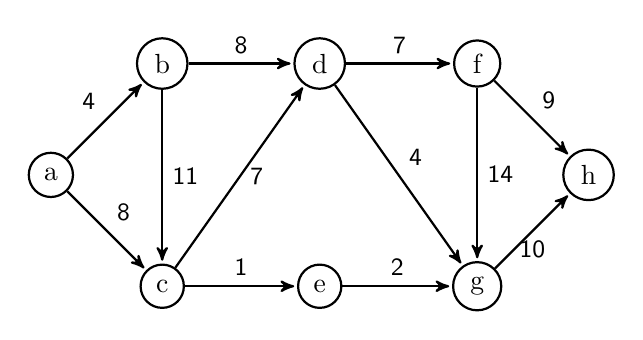
\begin{tikzpicture}[->,>=stealth',shorten >=1pt,auto,node distance=2cm,
	thick,main node/.style={circle,draw}]
	
	\node[main node] (a) {a};
	\node[main node] (b) [above right of=a] {b};
	\node[main node] (c) [below right of=a] {c};
	\node[main node] (d) [right of=b] {d};
	\node[main node] (e) [right of=c] {e};
	\node[main node] (f) [right of=d] {f};
	\node[main node] (g) [right of=e] {g};
	\node[main node] (h) [above right of=g] {h};
	
	\path[every node/.style={font=\sffamily\small}]
	(a) edge node [] {4} (b)
	(a)	edge node [] {8} (c)
	(b)	edge node [] {11} (c)
	(b) edge node [] {8} (d)
	(c)	edge node [] {1} (e)
	(c)	edge node [right] {7} (d)
	(d) edge node [] {7} (f)
	(d) edge node [] {4} (g)
	(e) edge node [] {2} (g)
	(f) edge node [] {14} (g)
	(f) edge node [] {9} (h)
	(g) edge node [below] {10} (h);
	\end{tikzpicture}
\end{figure}

\subsubsection*{Initialization}

\begin{minipage}{0.50\linewidth}
	\begin{tabular}{| c |  >{$}c<{$} | >{$}c<{$} |c|}
		\hline
		Vertex	&	\text{Distance}	&	\text{Source}	&	Visited\\
		\hline
		a		&	0				&	nil				&	\\
		\hline
		b		&	\infty			&	nil				&	\\
		\hline
		c		&	\infty			&	nil				&	\\
		\hline
		d		&	\infty			&	nil				&	\\
		\hline
		e		&	\infty			&	nil				&	\\
		\hline
		f		&	\infty			&	nil				&	\\
		\hline
		g		&	\infty			&	nil				&	\\
		\hline
		h		&	\infty			&	nil				&	\\
		\hline
	\end{tabular}
\end{minipage}
\qquad
\begin{minipage}{0.50\linewidth}
\begin{figure}[H]
	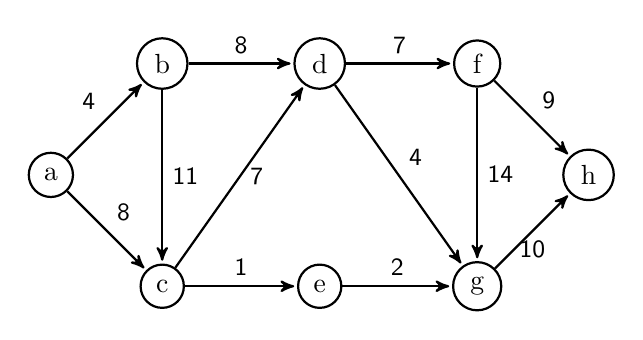
\begin{tikzpicture}[->,>=stealth',shorten >=1pt,auto,node distance=2cm,
	thick,main node/.style={circle,draw}]
	
	\node[main node] (a) {a};
	\node[main node] (b) [above right of=a] {b};
	\node[main node] (c) [below right of=a] {c};
	\node[main node] (d) [right of=b] {d};
	\node[main node] (e) [right of=c] {e};
	\node[main node] (f) [right of=d] {f};
	\node[main node] (g) [right of=e] {g};
	\node[main node] (h) [above right of=g] {h};
	
	\path[every node/.style={font=\sffamily\small}]
	(a) edge node [] {4} (b)
	(a)	edge node [] {8} (c)
	(b)	edge node [] {11} (c)
	(b) edge node [] {8} (d)
	(c)	edge node [] {1} (e)
	(c)	edge node [right] {7} (d)
	(d) edge node [] {7} (f)
	(d) edge node [] {4} (g)
	(e) edge node [] {2} (g)
	(f) edge node [] {14} (g)
	(f) edge node [] {9} (h)
	(g) edge node [below] {10} (h);
	\end{tikzpicture}
\end{figure}
\end{minipage}

\subsubsection*{Visit Vertex a}

\begin{minipage}{0.50\linewidth}
	\begin{tabular}{| c |  >{$}c<{$} | >{$}c<{$} |c|}
		\hline
		Vertex	&	\text{Distance}	&	\text{Source}	&	Visited\\
		\hline
		a		&	0				&	nil				&	x\\
		\hline
		b		&	4				&	a				&	\\
		\hline
		c		&	8				&	a				&	\\
		\hline
		d		&	\infty			&	nil				&	\\
		\hline
		e		&	\infty			&	nil				&	\\
		\hline
		f		&	\infty			&	nil				&	\\
		\hline
		g		&	\infty			&	nil				&	\\
		\hline
		h		&	\infty			&	nil				&	\\
		\hline
	\end{tabular}
\end{minipage}
\qquad
\begin{minipage}{0.50\linewidth}
	\begin{figure}[H]
		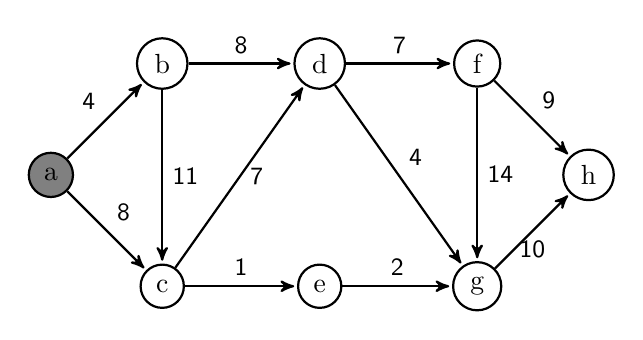
\begin{tikzpicture}[->,>=stealth',shorten >=1pt,auto,node distance=2cm,
		thick,main node/.style={circle,draw}]
		
		\node[main node, fill=gray] (a) {a};
		\node[main node] (b) [above right of=a] {b};
		\node[main node] (c) [below right of=a] {c};
		\node[main node] (d) [right of=b] {d};
		\node[main node] (e) [right of=c] {e};
		\node[main node] (f) [right of=d] {f};
		\node[main node] (g) [right of=e] {g};
		\node[main node] (h) [above right of=g] {h};
		
		\path[every node/.style={font=\sffamily\small}]
		(a) edge node [] {4} (b)
		(a)	edge node [] {8} (c)
		(b)	edge node [] {11} (c)
		(b) edge node [] {8} (d)
		(c)	edge node [] {1} (e)
		(c)	edge node [right] {7} (d)
		(d) edge node [] {7} (f)
		(d) edge node [] {4} (g)
		(e) edge node [] {2} (g)
		(f) edge node [] {14} (g)
		(f) edge node [] {9} (h)
		(g) edge node [below] {10} (h);
		\end{tikzpicture}
	\end{figure}
\end{minipage}

\subsubsection*{Visit Vertex b}

\begin{minipage}{0.50\linewidth}
	\begin{tabular}{| c |  >{$}c<{$} | >{$}c<{$} |c|}
		\hline
		Vertex	&	\text{Distance}	&	\text{Source}	&	Visited\\
		\hline
		a		&	0				&	nil				&	x\\
		\hline
		b		&	4				&	a				&	x\\
		\hline
		c		&	8				&	a				&	\\
		\hline
		d		&	12				&	b				&	\\
		\hline
		e		&	\infty			&	nil				&	\\
		\hline
		f		&	\infty			&	nil				&	\\
		\hline
		g		&	\infty			&	nil				&	\\
		\hline
		h		&	\infty			&	nil				&	\\
		\hline
	\end{tabular}
\end{minipage}
\qquad
\begin{minipage}{0.50\linewidth}
	\begin{figure}[H]
		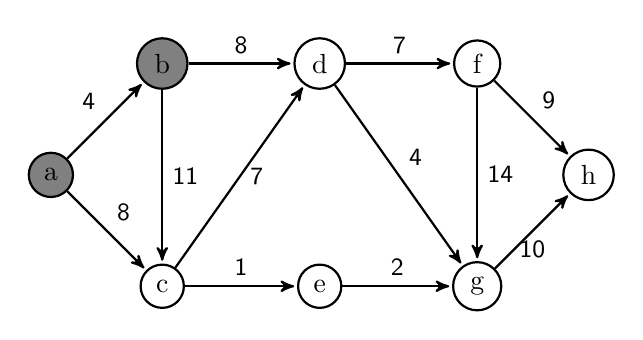
\begin{tikzpicture}[->,>=stealth',shorten >=1pt,auto,node distance=2cm,
		thick,main node/.style={circle,draw}]
		
		\node[main node, fill=gray] (a) {a};
		\node[main node, fill=gray] (b) [above right of=a] {b};
		\node[main node] (c) [below right of=a] {c};
		\node[main node] (d) [right of=b] {d};
		\node[main node] (e) [right of=c] {e};
		\node[main node] (f) [right of=d] {f};
		\node[main node] (g) [right of=e] {g};
		\node[main node] (h) [above right of=g] {h};
		
		\path[every node/.style={font=\sffamily\small}]
		(a) edge node [] {4} (b)
		(a)	edge node [] {8} (c)
		(b)	edge node [] {11} (c)
		(b) edge node [] {8} (d)
		(c)	edge node [] {1} (e)
		(c)	edge node [right] {7} (d)
		(d) edge node [] {7} (f)
		(d) edge node [] {4} (g)
		(e) edge node [] {2} (g)
		(f) edge node [] {14} (g)
		(f) edge node [] {9} (h)
		(g) edge node [below] {10} (h);
		\end{tikzpicture}
	\end{figure}
\end{minipage}

\subsubsection*{Visit Vertex c}

\begin{minipage}{0.50\linewidth}
	\begin{tabular}{| c |  >{$}c<{$} | >{$}c<{$} |c|}
		\hline
		Vertex	&	\text{Distance}	&	\text{Source}	&	Visited\\
		\hline
		a		&	0				&	nil				&	x\\
		\hline
		b		&	4				&	a				&	x\\
		\hline
		c		&	8				&	a				&	x\\
		\hline
		d		&	12				&	b				&	\\
		\hline
		e		&	9				&	c				&	\\
		\hline
		f		&	\infty			&	nil				&	\\
		\hline
		g		&	\infty			&	nil				&	\\
		\hline
		h		&	\infty			&	nil				&	\\
		\hline
	\end{tabular}
\end{minipage}
\qquad
\begin{minipage}{0.50\linewidth}
	\begin{figure}[H]
		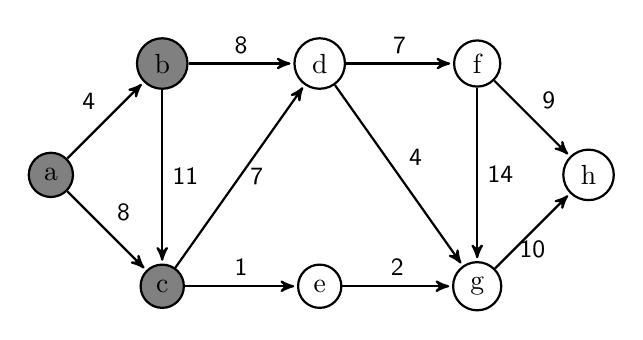
\begin{tikzpicture}[->,>=stealth',shorten >=1pt,auto,node distance=2cm,
		thick,main node/.style={circle,draw}]
		
		\node[main node, fill=gray] (a) {a};
		\node[main node, fill=gray] (b) [above right of=a] {b};
		\node[main node, fill=gray] (c) [below right of=a] {c};
		\node[main node] (d) [right of=b] {d};
		\node[main node] (e) [right of=c] {e};
		\node[main node] (f) [right of=d] {f};
		\node[main node] (g) [right of=e] {g};
		\node[main node] (h) [above right of=g] {h};
		
		\path[every node/.style={font=\sffamily\small}]
		(a) edge node [] {4} (b)
		(a)	edge node [] {8} (c)
		(b)	edge node [] {11} (c)
		(b) edge node [] {8} (d)
		(c)	edge node [] {1} (e)
		(c)	edge node [right] {7} (d)
		(d) edge node [] {7} (f)
		(d) edge node [] {4} (g)
		(e) edge node [] {2} (g)
		(f) edge node [] {14} (g)
		(f) edge node [] {9} (h)
		(g) edge node [below] {10} (h);
		\end{tikzpicture}
	\end{figure}
\end{minipage}

\subsubsection*{Visit Vertex e}

\begin{minipage}{0.50\linewidth}
	\begin{tabular}{| c |  >{$}c<{$} | >{$}c<{$} |c|}
		\hline
		Vertex	&	\text{Distance}	&	\text{Source}	&	Visited\\
		\hline
		a		&	0				&	nil				&	x\\
		\hline
		b		&	4				&	a				&	x\\
		\hline
		c		&	8				&	a				&	x\\
		\hline
		d		&	12				&	b				&	\\
		\hline
		e		&	9				&	c				&	x\\
		\hline
		f		&	\infty			&	nil				&	\\
		\hline
		g		&	11				&	e				&	\\
		\hline
		h		&	\infty			&	nil				&	\\
		\hline
	\end{tabular}
\end{minipage}
\qquad
\begin{minipage}{0.50\linewidth}
	\begin{figure}[H]
		\begin{tikzpicture}[->,>=stealth',shorten >=1pt,auto,node distance=2cm,
		thick,main node/.style={circle,draw}]
		
		\node[main node, fill=gray] (a) {a};
		\node[main node, fill=gray] (b) [above right of=a] {b};
		\node[main node, fill=gray] (c) [below right of=a] {c};
		\node[main node] (d) [right of=b] {d};
		\node[main node, fill=gray] (e) [right of=c] {e};
		\node[main node] (f) [right of=d] {f};
		\node[main node] (g) [right of=e] {g};
		\node[main node] (h) [above right of=g] {h};
		
		\path[every node/.style={font=\sffamily\small}]
		(a) edge node [] {4} (b)
		(a)	edge node [] {8} (c)
		(b)	edge node [] {11} (c)
		(b) edge node [] {8} (d)
		(c)	edge node [] {1} (e)
		(c)	edge node [right] {7} (d)
		(d) edge node [] {7} (f)
		(d) edge node [] {4} (g)
		(e) edge node [] {2} (g)
		(f) edge node [] {14} (g)
		(f) edge node [] {9} (h)
		(g) edge node [below] {10} (h);
		\end{tikzpicture}
	\end{figure}
\end{minipage}

\subsubsection*{Visit Vertex g}

\begin{minipage}{0.50\linewidth}
	\begin{tabular}{| c |  >{$}c<{$} | >{$}c<{$} |c|}
		\hline
		Vertex	&	\text{Distance}	&	\text{Source}	&	Visited\\
		\hline
		a		&	0				&	nil				&	x\\
		\hline
		b		&	4				&	a				&	x\\
		\hline
		c		&	8				&	a				&	x\\
		\hline
		d		&	12				&	b				&	\\
		\hline
		e		&	9				&	c				&	x\\
		\hline
		f		&	\infty			&	nil				&	\\
		\hline
		g		&	11				&	e				&	x\\
		\hline
		h		&	21				&	g				&	\\
		\hline
	\end{tabular}
\end{minipage}
\qquad
\begin{minipage}{0.50\linewidth}
	\begin{figure}[H]
		\begin{tikzpicture}[->,>=stealth',shorten >=1pt,auto,node distance=2cm,
		thick,main node/.style={circle,draw}]
		
		\node[main node, fill=gray] (a) {a};
		\node[main node, fill=gray] (b) [above right of=a] {b};
		\node[main node, fill=gray] (c) [below right of=a] {c};
		\node[main node] (d) [right of=b] {d};
		\node[main node, fill=gray] (e) [right of=c] {e};
		\node[main node] (f) [right of=d] {f};
		\node[main node, fill=gray] (g) [right of=e] {g};
		\node[main node] (h) [above right of=g] {h};
		
		\path[every node/.style={font=\sffamily\small}]
		(a) edge node [] {4} (b)
		(a)	edge node [] {8} (c)
		(b)	edge node [] {11} (c)
		(b) edge node [] {8} (d)
		(c)	edge node [] {1} (e)
		(c)	edge node [right] {7} (d)
		(d) edge node [] {7} (f)
		(d) edge node [] {4} (g)
		(e) edge node [] {2} (g)
		(f) edge node [] {14} (g)
		(f) edge node [] {9} (h)
		(g) edge node [below] {10} (h);
		\end{tikzpicture}
	\end{figure}
\end{minipage}

\subsubsection*{Visit Vertex d}

\begin{minipage}{0.50\linewidth}
	\begin{tabular}{| c |  >{$}c<{$} | >{$}c<{$} |c|}
		\hline
		Vertex	&	\text{Distance}	&	\text{Source}	&	Visited\\
		\hline
		a		&	0				&	nil				&	x\\
		\hline
		b		&	4				&	a				&	x\\
		\hline
		c		&	8				&	a				&	x\\
		\hline
		d		&	12				&	b				&	x\\
		\hline
		e		&	9				&	c				&	x\\
		\hline
		f		&	19				&	d				&	\\
		\hline
		g		&	11				&	e				&	x\\
		\hline
		h		&	21				&	g				&	\\
		\hline
	\end{tabular}
\end{minipage}
\qquad
\begin{minipage}{0.50\linewidth}
	\begin{figure}[H]
		\begin{tikzpicture}[->,>=stealth',shorten >=1pt,auto,node distance=2cm,
		thick,main node/.style={circle,draw}]
		
		\node[main node, fill=gray] (a) {a};
		\node[main node, fill=gray] (b) [above right of=a] {b};
		\node[main node, fill=gray] (c) [below right of=a] {c};
		\node[main node, fill=gray] (d) [right of=b] {d};
		\node[main node, fill=gray] (e) [right of=c] {e};
		\node[main node] (f) [right of=d] {f};
		\node[main node, fill=gray] (g) [right of=e] {g};
		\node[main node] (h) [above right of=g] {h};
		
		\path[every node/.style={font=\sffamily\small}]
		(a) edge node [] {4} (b)
		(a)	edge node [] {8} (c)
		(b)	edge node [] {11} (c)
		(b) edge node [] {8} (d)
		(c)	edge node [] {1} (e)
		(c)	edge node [right] {7} (d)
		(d) edge node [] {7} (f)
		(d) edge node [] {4} (g)
		(e) edge node [] {2} (g)
		(f) edge node [] {14} (g)
		(f) edge node [] {9} (h)
		(g) edge node [below] {10} (h);
		\end{tikzpicture}
	\end{figure}
\end{minipage}

\subsubsection*{Visit Vertex f}

\begin{minipage}{0.50\linewidth}
	\begin{tabular}{| c |  >{$}c<{$} | >{$}c<{$} |c|}
		\hline
		Vertex	&	\text{Distance}	&	\text{Source}	&	Visited\\
		\hline
		a		&	0				&	nil				&	x\\
		\hline
		b		&	4				&	a				&	x\\
		\hline
		c		&	8				&	a				&	x\\
		\hline
		d		&	12				&	b				&	x\\
		\hline
		e		&	9				&	c				&	x\\
		\hline
		f		&	19				&	d				&	x\\
		\hline
		g		&	11				&	e				&	x\\
		\hline
		h		&	21				&	g				&	\\
		\hline
	\end{tabular}
\end{minipage}
\qquad
\begin{minipage}{0.50\linewidth}
	\begin{figure}[H]
		\begin{tikzpicture}[->,>=stealth',shorten >=1pt,auto,node distance=2cm,
		thick,main node/.style={circle,draw}]
		
		\node[main node, fill=gray] (a) {a};
		\node[main node, fill=gray] (b) [above right of=a] {b};
		\node[main node, fill=gray] (c) [below right of=a] {c};
		\node[main node, fill=gray] (d) [right of=b] {d};
		\node[main node, fill=gray] (e) [right of=c] {e};
		\node[main node, fill=gray] (f) [right of=d] {f};
		\node[main node, fill=gray] (g) [right of=e] {g};
		\node[main node] (h) [above right of=g] {h};
		
		\path[every node/.style={font=\sffamily\small}]
		(a) edge node [] {4} (b)
		(a)	edge node [] {8} (c)
		(b)	edge node [] {11} (c)
		(b) edge node [] {8} (d)
		(c)	edge node [] {1} (e)
		(c)	edge node [right] {7} (d)
		(d) edge node [] {7} (f)
		(d) edge node [] {4} (g)
		(e) edge node [] {2} (g)
		(f) edge node [] {14} (g)
		(f) edge node [] {9} (h)
		(g) edge node [below] {10} (h);
		\end{tikzpicture}
	\end{figure}
\end{minipage}

\subsubsection*{Visit Vertex h}

\begin{minipage}{0.50\linewidth}
	\begin{tabular}{| c |  >{$}c<{$} | >{$}c<{$} |c|}
		\hline
		Vertex	&	\text{Distance}	&	\text{Source}	&	Visited\\
		\hline
		a		&	0				&	nil				&	x\\
		\hline
		b		&	4				&	a				&	x\\
		\hline
		c		&	8				&	a				&	x\\
		\hline
		d		&	12				&	b				&	x\\
		\hline
		e		&	9				&	c				&	x\\
		\hline
		f		&	19				&	d				&	x\\
		\hline
		g		&	11				&	e				&	x\\
		\hline
		h		&	21				&	g				&	x\\
		\hline
	\end{tabular}
\end{minipage}
\qquad
\begin{minipage}{0.50\linewidth}
	\begin{figure}[H]
		\begin{tikzpicture}[->,>=stealth',shorten >=1pt,auto,node distance=2cm,
		thick,main node/.style={circle,draw}]
		
		\node[main node, fill=gray] (a) {a};
		\node[main node, fill=gray] (b) [above right of=a] {b};
		\node[main node, fill=gray] (c) [below right of=a] {c};
		\node[main node, fill=gray] (d) [right of=b] {d};
		\node[main node, fill=gray] (e) [right of=c] {e};
		\node[main node, fill=gray] (f) [right of=d] {f};
		\node[main node, fill=gray] (g) [right of=e] {g};
		\node[main node, fill=gray] (h) [above right of=g] {h};
		
		\path[every node/.style={font=\sffamily\small}]
		(a) edge node [] {4} (b)
		(a)	edge node [] {8} (c)
		(b)	edge node [] {11} (c)
		(b) edge node [] {8} (d)
		(c)	edge node [] {1} (e)
		(c)	edge node [right] {7} (d)
		(d) edge node [] {7} (f)
		(d) edge node [] {4} (g)
		(e) edge node [] {2} (g)
		(f) edge node [] {14} (g)
		(f) edge node [] {9} (h)
		(g) edge node [below] {10} (h);
		\end{tikzpicture}
	\end{figure}
\end{minipage}

\subsubsection*{Solution}
	\begin{figure}[H]
		\centering
		\begin{tikzpicture}[->,>=stealth',shorten >=1pt,auto,node distance=2cm,
		thick,main node/.style={circle,draw}]
		
		\node[main node] (a) {a};
		\node[main node] (b) [above right of=a] {b};
		\node[main node] (c) [below right of=a] {c};
		\node[main node] (d) [right of=b] {d};
		\node[main node] (e) [right of=c] {e};
		\node[main node] (f) [right of=d] {f};
		\node[main node] (g) [right of=e] {g};
		\node[main node] (h) [above right of=g] {h};
		
		\path[every node/.style={font=\sffamily\small}]
		(a) edge node [] {4} (b)
		(a)	edge node [] {8} (c)
		(b) edge node [] {8} (d)
		(c)	edge node [] {1} (e)
		(d) edge node [] {7} (f)
		(e) edge node [] {2} (g)
		(g) edge node [below] {10} (h);
		\end{tikzpicture}
	\end{figure}
\newpage

\section{Bellman-Ford Algorithm}

\subsection*{Steps}
\begin{enumerate}
	\item For every vertex $v \in V$, if the vertex is starting vertex then set its distance to 0. Otherwise, set its distance to $\infty$.
	\item Also for every vertex $v \in V$, set the source to $nil$.
	\item Repeat the following process $\vert V \vert - 1$ times:
	\begin{enumerate}
		\item For every edge $e = (u,v) \in E$ with weight $w$, calculate the $\text{candidate} = \text{distance}(u) + w$.
		\item If candidate $< \text{distance}(v)$, then $\text{distance}(v) = \text{candidate}$ and source($v$) = $u$.
		\item Otherwise, $\text{distance}(v)$ remains the same.\\
			Essentially: $\text{distance}(v) = \min\{ \text{distance}(u) + w, \text{distance}(v)   \}$
	\end{enumerate}
	\item Lastly, check for negative-weight cycles:
	\begin{enumerate}
		\item For every edge $e = (u,v) \in E$, calculate: $\text{distance}(u) + w$. If this sum is less than $\text{distance}(v)$ then the graph contains a negative-weight cycle.
		\item Return FALSE on negative-weight cycle.
	\end{enumerate}
\end{enumerate}

\subsection*{Complexity}
$$
O(\vert V \vert \vert E \vert)
$$

\newpage

\subsection{Example}
\textbf{Given the following graph $G$, perform Bellman-Ford algorithm starting from vertex $a$.}\\
***Assume all edges are processed in lexical order: $(a,b), (a,c), (b,c), (b,d), (c,d), (c,e), (d,f), (d,g), (f,g), (f,h), (g,h)$

\begin{figure}[H]
	\centering
	\begin{tikzpicture}[->,>=stealth',shorten >=1pt,auto,node distance=2cm,
	thick,main node/.style={circle,draw}]
	
	\node[main node] (a) {a};
	\node[main node] (b) [above right of=a] {b};
	\node[main node] (c) [below right of=a] {c};
	\node[main node] (d) [right of=b] {d};
	\node[main node] (e) [right of=c] {e};
	\node[main node] (f) [right of=d] {f};
	\node[main node] (g) [right of=e] {g};
	\node[main node] (h) [above right of=g] {h};
	
	\path[every node/.style={font=\sffamily\small}]
	(a) edge node [] {4} (b)
	(a)	edge node [] {8} (c)
	(b)	edge node [] {11} (c)
	(b) edge node [] {8} (d)
	(c)	edge node [] {1} (e)
	(c)	edge node [right] {7} (d)
	(d) edge node [] {7} (f)
	(d) edge node [] {4} (g)
	(f) edge node [] {14} (g)
	(f) edge node [] {9} (h)
	(g) edge node [below] {10} (h)
	(g) edge node [] {-10} (e);
	\end{tikzpicture}
\end{figure}

\subsubsection*{Initialization}

\begin{minipage}{0.50\linewidth}
	\begin{tabular}{| c |  >{$}c<{$} | >{$}c<{$} |}
		\hline
		Vertex	&	\text{Distance}	&	\text{Source}\\
		\hline
		a		&	0				&	nil				\\
		\hline
		b		&	\infty			&	nil				\\
		\hline
		c		&	\infty			&	nil				\\
		\hline
		d		&	\infty			&	nil				\\
		\hline
		e		&	\infty			&	nil				\\
		\hline
		f		&	\infty			&	nil				\\
		\hline
		g		&	\infty			&	nil				\\
		\hline
		h		&	\infty			&	nil				\\
		\hline
	\end{tabular}
\end{minipage}
\qquad
\begin{minipage}{0.50\linewidth}
	\begin{figure}[H]
		\begin{tikzpicture}[->,>=stealth',shorten >=1pt,auto,node distance=2cm,
		thick,main node/.style={circle,draw}]
		
		\node[main node] (a) {$a_0$};
		\node[main node] (b) [above right of=a] {$b_\infty$};
		\node[main node] (c) [below right of=a] {$c_\infty$};
		\node[main node] (d) [right of=b] {$d_\infty$};
		\node[main node] (e) [right of=c] {$e_\infty$};
		\node[main node] (f) [right of=d] {$f_\infty$};
		\node[main node] (g) [right of=e] {$g_\infty$};
		\node[main node] (h) [above right of=g] {$h_\infty$};
		
	\path[every node/.style={font=\sffamily\small}]
	(a) edge node [] {4} (b)
	(a)	edge node [] {8} (c)
	(b)	edge node [] {11} (c)
	(b) edge node [] {8} (d)
	(c)	edge node [] {1} (e)
	(c)	edge node [right] {7} (d)
	(d) edge node [] {7} (f)
	(d) edge node [] {4} (g)
	(f) edge node [] {14} (g)
	(f) edge node [] {9} (h)
	(g) edge node [below] {10} (h)
	(g) edge node [] {-10} (e);
		\end{tikzpicture}
	\end{figure}
\end{minipage}

\subsubsection*{Iteration 1}

\begin{minipage}{0.50\linewidth}
	\begin{tabular}{| c |  >{$}c<{$} | >{$}c<{$} |}
		\hline
		Vertex	&	\text{Distance}	&	\text{Source}\\
		\hline
		a		&	0				&	nil				\\
		\hline
		b		&	4				&	a				\\
		\hline
		c		&	8				&	a				\\
		\hline
		d		&	\infty				&	nil				\\
		\hline
		e		&	\infty				&	nil			\\
		\hline
		f		&	\infty			&	nil				\\
		\hline
		g		&	\infty			&	nil				\\
		\hline
		h		&	\infty			&	nil				\\
		\hline
	\end{tabular}
\end{minipage}
\qquad
\begin{minipage}{0.50\linewidth}
	\begin{figure}[H]
		\begin{tikzpicture}[->,>=stealth',shorten >=1pt,auto,node distance=2cm,
		thick,main node/.style={circle,draw}]
		
		\node[main node] (a) {$a_0$};
		\node[main node] (b) [above right of=a] {$b_4$};
		\node[main node] (c) [below right of=a] {$c_8$};
		\node[main node] (d) [right of=b] {$d_{\infty}$};
		\node[main node] (e) [right of=c] {$e_\infty$};
		\node[main node] (f) [right of=d] {$f_\infty$};
		\node[main node] (g) [right of=e] {$g_\infty$};
		\node[main node] (h) [above right of=g] {$h_\infty$};

	\path[every node/.style={font=\sffamily\small}]
	(a) edge node [] {4} (b)
	(a)	edge node [] {8} (c)
	(b)	edge node [] {11} (c)
	(b) edge node [] {8} (d)
	(c)	edge node [] {1} (e)
	(c)	edge node [right] {7} (d)
	(d) edge node [] {7} (f)
	(d) edge node [] {4} (g)
	(f) edge node [] {14} (g)
	(f) edge node [] {9} (h)
	(g) edge node [below] {10} (h)
	(g) edge node [] {-10} (e);
		\end{tikzpicture}
	\end{figure}
\end{minipage}

\subsubsection*{Iteration 2}

\begin{minipage}{0.50\linewidth}
	\begin{tabular}{| c |  >{$}c<{$} | >{$}c<{$} |}
		\hline
		Vertex	&	\text{Distance}	&	\text{Source}\\
		\hline
		a		&	0				&	nil				\\
		\hline
		b		&	4				&	a				\\
		\hline
		c		&	8				&	a				\\
		\hline
		d		&	12				&	b				\\
		\hline
		e		&	9				&	c			\\
		\hline
		f		&	\infty			&	nil				\\
		\hline
		g		&	\infty			&	nil				\\
		\hline
		h		&	\infty			&	nil				\\
		\hline
	\end{tabular}
\end{minipage}
\qquad
\begin{minipage}{0.50\linewidth}
	\begin{figure}[H]
		\begin{tikzpicture}[->,>=stealth',shorten >=1pt,auto,node distance=2cm,
		thick,main node/.style={circle,draw}]
		
		\node[main node] (a) {$a_0$};
		\node[main node] (b) [above right of=a] {$b_4$};
		\node[main node] (c) [below right of=a] {$c_8$};
		\node[main node] (d) [right of=b] {$d_{12}$};
		\node[main node] (e) [right of=c] {$e_9$};
		\node[main node] (f) [right of=d] {$f_\infty$};
		\node[main node] (g) [right of=e] {$g_\infty$};
		\node[main node] (h) [above right of=g] {$h_\infty$};
		
	\path[every node/.style={font=\sffamily\small}]
	(a) edge node [] {4} (b)
	(a)	edge node [] {8} (c)
	(b)	edge node [] {11} (c)
	(b) edge node [] {8} (d)
	(c)	edge node [] {1} (e)
	(c)	edge node [right] {7} (d)
	(d) edge node [] {7} (f)
	(d) edge node [] {4} (g)
	(f) edge node [] {14} (g)
	(f) edge node [] {9} (h)
	(g) edge node [below] {10} (h)
	(g) edge node [] {-10} (e);
		\end{tikzpicture}
	\end{figure}
\end{minipage}

\subsubsection*{Iteration 3}

\begin{minipage}{0.50\linewidth}
	\begin{tabular}{| c |  >{$}c<{$} | >{$}c<{$} |}
		\hline
		Vertex	&	\text{Distance}	&	\text{Source}\\
		\hline
		a		&	0				&	nil				\\
		\hline
		b		&	4				&	a				\\
		\hline
		c		&	8				&	a				\\
		\hline
		d		&	12				&	b				\\
		\hline
		e		&	9				&	c			\\
		\hline
		f		&	19				&	d				\\
		\hline
		g		&	16				&	d				\\
		\hline
		h		&	\infty			&	nil				\\
		\hline
	\end{tabular}
\end{minipage}
\qquad
\begin{minipage}{0.50\linewidth}
	\begin{figure}[H]
		\begin{tikzpicture}[->,>=stealth',shorten >=1pt,auto,node distance=2cm,
		thick,main node/.style={circle,draw}]
		
		\node[main node] (a) {$a_0$};
		\node[main node] (b) [above right of=a] {$b_4$};
		\node[main node] (c) [below right of=a] {$c_8$};
		\node[main node] (d) [right of=b] {$d_{12}$};
		\node[main node] (e) [right of=c] {$e_9$};
		\node[main node] (f) [right of=d] {$f_{19}$};
		\node[main node] (g) [right of=e] {$g_{16}$};
		\node[main node] (h) [above right of=g] {$h_\infty$};
		
		\path[every node/.style={font=\sffamily\small}]
		(a) edge node [] {4} (b)
		(a)	edge node [] {8} (c)
		(b)	edge node [] {11} (c)
		(b) edge node [] {8} (d)
		(c)	edge node [] {1} (e)
		(c)	edge node [right] {7} (d)
		(d) edge node [] {7} (f)
		(d) edge node [] {4} (g)
		(f) edge node [] {14} (g)
		(f) edge node [] {9} (h)
		(g) edge node [below] {10} (h)
		(g) edge node [] {-10} (e);
		\end{tikzpicture}
	\end{figure}
\end{minipage}

\subsubsection*{Iteration 4}

\begin{minipage}{0.50\linewidth}
	\begin{tabular}{| c |  >{$}c<{$} | >{$}c<{$} |}
		\hline
		Vertex	&	\text{Distance}	&	\text{Source}\\
		\hline
		a		&	0				&	nil				\\
		\hline
		b		&	4				&	a				\\
		\hline
		c		&	8				&	a				\\
		\hline
		d		&	12				&	b				\\
		\hline
		e		&	6				&	g			\\
		\hline
		f		&	19				&	d				\\
		\hline
		g		&	16				&	d				\\
		\hline
		h		&	26				&	g				\\
		\hline
	\end{tabular}
\end{minipage}
\qquad
\begin{minipage}{0.50\linewidth}
	\begin{figure}[H]
		\begin{tikzpicture}[->,>=stealth',shorten >=1pt,auto,node distance=2cm,
		thick,main node/.style={circle,draw}]
		
		\node[main node] (a) {$a_0$};
		\node[main node] (b) [above right of=a] {$b_4$};
		\node[main node] (c) [below right of=a] {$c_8$};
		\node[main node] (d) [right of=b] {$d_{12}$};
		\node[main node] (e) [right of=c] {$e_6$};
		\node[main node] (f) [right of=d] {$f_{19}$};
		\node[main node] (g) [right of=e] {$g_{16}$};
		\node[main node] (h) [above right of=g] {$h_{26}$};
		
		\path[every node/.style={font=\sffamily\small}]
		(a) edge node [] {4} (b)
		(a)	edge node [] {8} (c)
		(b)	edge node [] {11} (c)
		(b) edge node [] {8} (d)
		(c)	edge node [] {1} (e)
		(c)	edge node [right] {7} (d)
		(d) edge node [] {7} (f)
		(d) edge node [] {4} (g)
		(f) edge node [] {14} (g)
		(f) edge node [] {9} (h)
		(g) edge node [below] {10} (h)
		(g) edge node [] {-10} (e);
		\end{tikzpicture}
	\end{figure}
\end{minipage}

\subsubsection*{Iteration 5,6,7}

\begin{minipage}{0.50\linewidth}
	\begin{tabular}{| c |  >{$}c<{$} | >{$}c<{$} |}
		\hline
		Vertex	&	\text{Distance}	&	\text{Source}\\
		\hline
		a		&	0				&	nil				\\
		\hline
		b		&	4				&	a				\\
		\hline
		c		&	8				&	a				\\
		\hline
		d		&	12				&	b				\\
		\hline
		e		&	6				&	g			\\
		\hline
		f		&	19				&	d				\\
		\hline
		g		&	16				&	d				\\
		\hline
		h		&	26				&	g				\\
		\hline
	\end{tabular}
\end{minipage}
\qquad
\begin{minipage}{0.50\linewidth}
	\begin{figure}[H]
		\begin{tikzpicture}[->,>=stealth',shorten >=1pt,auto,node distance=2cm,
		thick,main node/.style={circle,draw}]
		
		\node[main node] (a) {$a_0$};
		\node[main node] (b) [above right of=a] {$b_4$};
		\node[main node] (c) [below right of=a] {$c_8$};
		\node[main node] (d) [right of=b] {$d_{12}$};
		\node[main node] (e) [right of=c] {$e_6$};
		\node[main node] (f) [right of=d] {$f_{19}$};
		\node[main node] (g) [right of=e] {$g_{16}$};
		\node[main node] (h) [above right of=g] {$h_{26}$};
		
		\path[every node/.style={font=\sffamily\small}]
		(a) edge node [] {4} (b)
		(a)	edge node [] {8} (c)
		(b)	edge node [] {11} (c)
		(b) edge node [] {8} (d)
		(c)	edge node [] {1} (e)
		(c)	edge node [right] {7} (d)
		(d) edge node [] {7} (f)
		(d) edge node [] {4} (g)
		(f) edge node [] {14} (g)
		(f) edge node [] {9} (h)
		(g) edge node [below] {10} (h)
		(g) edge node [] {-10} (e);
		\end{tikzpicture}
	\end{figure}
\end{minipage}

\subsubsection*{Solution}
	\begin{figure}[H]
		\centering
		\begin{tikzpicture}[->,>=stealth',shorten >=1pt,auto,node distance=2cm,
		thick,main node/.style={circle,draw}]
		
		\node[main node] (a) {$a$};
		\node[main node] (b) [above right of=a] {$b$};
		\node[main node] (c) [below right of=a] {$c$};
		\node[main node] (d) [right of=b] {$d$};
		\node[main node] (e) [right of=c] {$e$};
		\node[main node] (f) [right of=d] {$f$};
		\node[main node] (g) [right of=e] {$g$};
		\node[main node] (h) [above right of=g] {$h$};
		
		\path[every node/.style={font=\sffamily\small}]
		(a) edge node [] {4} (b)
		(a)	edge node [] {8} (c)
		(b) edge node [] {8} (d)
		(d) edge node [] {7} (f)
		(d) edge node [] {4} (g)
		(g) edge node [below] {10} (h)
		(g) edge node [] {-10} (e);
		\end{tikzpicture}
	\end{figure}
\newpage

%
% APPENDIX
%
\chapter{Side Topics}
\newpage

\subsection{Solving Recurrence Relations with Induction}

\subsubsection{Example}
\textbf{Prove that the following systems of equations has the solution $T(n) = n \cdot lg(n)$.}
$$
T(n) \begin{cases}
	2T(\frac{n}{2}) + n, & n = 2^k \mbox{ for } k > 1\\
	2, & n = 2
\end{cases}
$$
\textbf{Basis}
\begin{eqnarray*}
T(2) &=& (2) \cdot lg(2)\\
	&=& 2 \cdot 1\\
	&=& 2
\end{eqnarray*}
\textbf{Inductive Hypothesis}\\
Assume that $T(n) = n \cdot lg(n)$ holds true for all $n = 2^k$.\\\\
\textbf{Inductive Step}
\begin{align*}
T(n)	&=	2T(\frac{n}{2}) + n						&& \text{Base equation}\\
		&= 	2T(\frac{2^{k+1}}{2}) + 2^{k+1}			&& \text{Substitute n with } 2^{k+1}\\
		&= 	2T(2^{k}) + 2^{k+1}						&& \text{Simplify parameters to function T(...)}\\
		&=	2(2^k \cdot lg(2^k)) + 2^{k+1}			&& \text{Inductive hypothesis}\\
		&=	2^{k+1} \left[ lg(2^k) + 1 \right]		&& \text{Distributive property}\\
		&=  2^{k+1} \left[ lg(2^k) + lg(2) \right]  && \text{Logarithmic identity}\\
		&= 	2^{k+1} \cdot lg(2^k \cdot 2)			&& \text{Logarithmic identity}\\
		&=  2^{k+1} \cdot lg(2^{k+1})				&& \text{Exponent property}\\
		&											&& \text{Q.E.D}
\end{align*}

\subsubsection{Example}
\textbf{Prove that the following systems of equations has the solution $T(n) = 2F(n) - 1$ where $F(n) = F(n-1) + F(n-2)$.}
$$
T(n) \begin{cases}
T(n-1) + T(n-2) + 1, & \mbox{if } n \geq 2\\
0, & \mbox{if } n = \{0,1\}
\end{cases}
$$
\textbf{Basis}
\begin{eqnarray*}
	T(0) &=& 1
\end{eqnarray*}
\textbf{Inductive Hypothesis}\\
Assume that $T(n) = F(n) - 1$ is true for all $n = k$.\\
\textbf{Inductive Step}
\begin{align*}
	T(n) 	&= T(n-1) + T(n-2) + 1					&& \text{Base equation}\\
	T(k+1) 	&= T((k+1) - 1) + T((k+1) - 2) + 1 		&& \text{Substitute n with k+1}\\
			&= T(k) + T(k-1) + 1					&& \text{Simplify parameters to function T(...)}\\
			&= (2F(k) - 1) + (2F(k-1) - 1) + 1		&& \text{Inductive hypothesis}\\
			&= 2F(k) + 2F(k-1) - 1					&& \text{Simplify equation}\\
			&= 2(F(k) + F(k-1)) - 1					&& \text{Distributive property}\\
			&= 2(F(k+1)) - 1						&& \text{Definition of function: } F(k+1) = F(k) + F(k-1)\\
			&= 2F(k+1) - 1							&& \text{Simplify}\\
			&										&& \text{Q.E.D}
\end{align*}


\end{document}